% 
% (c) Copyright 2016 Tabea Mendez
% 
% This source is free: you can redistribute it and/or modify
% it under the terms of the GNU General Public License as published by
% the Free Software Foundation, either version 3 of the License, or
% (at your option) any later version.
% 
% This source is distributed in the hope that it will be useful,
% but WITHOUT ANY WARRANTY; without even the implied warranty of
% MERCHANTABILITY or FITNESS FOR A PARTICULAR PURPOSE.  See the
% GNU General Public License for more details.
% 
% You should have received a copy of the GNU General Public License
% along with this source.  If not, see <http://www.gnu.org/licenses/>.
%
%%%%%%%%%%%%%%%%%%%%%%%%%%%%%%%%%%%%%%%%%%%%%%%%%%%%%%%%%%%%%%%%%%%%%%%%%%%%%%

\section{Interpolation und Oversampling}
	\begin{goal}
	  Ein Upsampling mit anschliessender Interpolation wird oft gemacht, um die Anforderungen an das analoge Anti-Image-Filter (D/A) zu verringern. Stattdessen wird jedoch ein digitales Interpolations-Filter mit hohen Anforderungen gebraucht.
	\end{goal}

	\subsection{Schritte im Zeitbereich}
		\hspace*{1cm}\includegraphics[width = 0.75\textwidth]{pic/Upsampler.pdf}
		\begin{itemize}
		  \item Digitales Signal $x(n)$ um den Faktor $L$ upsamplen, wobei alle neuen Samples auf Null gesetzt werden.\\[0.2cm]
		  \fcolorbox{CadetRed}{white}{$x_{up}(n') = \begin{cases}x(n),&\text{wenn }n' = n\, L\\ 0,&\text{sonst}\end{cases}$}$\qquad$mit$\qquad$\fcolorbox{CadetRed}{white}{$n' = n\,L + i$}$\quad i=0,1,2,...,L-1$\\
		  \item Das Upgesampletes Signal $x_{up}(n')$ wird durch ein\\FIR-Interpolations-Filter gelassen, welches die neuen\\ Samples auf den richtigen Wert setzt.\\[-1.35cm]
		  \hspace*{10.2cm}\fcolorbox{CadetRed}{white}{$y_{up}(n') = \mysum{k'}{\textcolor{white}{ds}}{h(k')\,x_{up}(n'-k')}$}\\[-0.1cm]
		  \item Es resultiert ein Signal $y_{up}(n')$ welches eine höhere Taktrate hat.$\qquad$
		  \fcolorbox{CadetRed}{white}{$f_s' = L\cdot f_s\qquad\Leftrightarrow\qquad T' = \dfrac{T}{L}$}\\[-0.4cm]
		\end{itemize}
		
	\subsection{Schritte im Frequenzbereich}
		\begin{itemize}
		  \item Spektrum $X(f)$ des langsam\\ abgetasteten Signal $x(n)$.\\[-1.5cm]
			\begin{minipage}{0.3\textwidth}$ $\end{minipage}
			\begin{minipage}{0.7\textwidth}
			\begin{tikzpicture}[>=latex, scale=0.9]
				\draw[->][line width=0.75](0,-0.2)node[below]{\small$0$}--(0,2.2)node[right]{\small$X(f)$};
				\draw[->][line width=0.75](-6,0)--(6,0)node[below]{\small$f$};

				\draw[line width=0.75](1.2,0.2)--(1.2,-0.2)node[below]{\small$f_s$};
				\draw[line width=0.75](-1.2,0.2)--(-1.2,-0.2)node[below]{\small$-f_s$};
				\draw[line width=0.75](2*1.2,0.2)--(2*1.2,-0.2)node[below]{\small$2f_s$};
				\draw[line width=0.75](-2*1.2,0.2)--(-2*1.2,-0.2)node[below]{\small$-2f_s$};
				\draw[line width=0.75](3*1.2,0.2)--(3*1.2,-0.2)node[below=5pt]{\small$\dots$};
				\draw[line width=0.75](-3*1.2,0.2)--(-3*1.2,-0.2)node[below=5pt]{\small$\dots$};
				\draw[line width=0.75](4*1.2,0.2)--(4*1.2,-0.2)node[below]{\small$Lf_s$};
				\draw[line width=0.75](-4*1.2,0.2)--(-4*1.2,-0.2)node[below]{\small$-Lf_s$};
				

				\foreach \i in {-4,...,4}
				{
					\draw[CadetRed, line width=1](1.2*\i,0)++(-0.6,0)--++(0.25,1.3)--node[above]{}++(0.7,0)--++(0.25,-1.3);
				}
				\draw[blueT, line width=1](0,0)++(-0.6,0)--++(0.25,1.3)--node[above left]{\small $f_s\,X_a(f)$}++(0.7,0)--++(0.25,-1.3);

				\draw[line width=2, blueT](-0.6,0)--(0.6,-0);
				\draw[line width=0.75, blueT](-0.6,0.2)--(-0.6,-0.9);
				\draw[line width=0.75, blueT](0.6,0.2)--(0.6,-0.9);
				\draw[line width=0.75, blueT,<->](-0.6,-0.8)--node[below]{\footnotesize Nyquistintervall}(0.6,-0.8);


				\begin{scope}[shift={(6,0)}]
					\draw[CadetRed, line width=1,fill](0,0.65)circle(1pt);
					\draw[CadetRed, line width=1,fill](0.25,0.65)circle(1pt);
					\draw[CadetRed, line width=1,fill](-0.25,0.65)circle(1pt);
				\end{scope}
				\begin{scope}[shift={(-6,0)}]
					\draw[CadetRed, line width=1,fill](0,0.65)circle(1pt);
					\draw[CadetRed, line width=1,fill](0.25,0.65)circle(1pt);
					\draw[CadetRed, line width=1,fill](-0.25,0.65)circle(1pt);
				\end{scope}
			\end{tikzpicture}	
			\end{minipage}\\[-0.4cm]
		  \item Durch das Upsamplen um den Faktor $L$ verändert sich\\ das Spektrum $X(f)$ des digitalen Signals $x(n)$\\ nicht, da die neuen Samples\\ alle Null sind. Es ändert nur\\ die Samplingfrequenz $f_s\rightarrow f_s'$\\[0.2cm]
		  $\;\Rightarrow\qquad$\fcolorbox{CadetRed}{white}{$X_{up}(f) = X(f)$}\\[-3.1cm]
			\begin{minipage}{0.3\textwidth}$ $\end{minipage}
			\begin{minipage}{0.7\textwidth}
			\begin{tikzpicture}[>=latex, scale=0.9]
				\draw[->][line width=0.75](0,-0.2)node[below]{\small$0$}--(0,2.2)node[right]{\small$X_{up}(f) = X(f)$};
				\draw[->][line width=0.75](-6,0)--(6,0)node[below]{\small$f$};

				\foreach \i in {-4,...,4}
				{
					\draw[CadetRed, line width=1](1.2*\i,0)++(-0.6,0)--++(0.25,1.3)--node[above]{}++(0.7,0)--++(0.25,-1.3);
				}
				\draw[blueT, line width=1](0,0)++(-0.6,0)--++(0.25,1.3)--node[above left]{\small $f_s\,X_a(f)$}++(0.7,0)--++(0.25,-1.3);

				\draw[line width=2, blueT](-0.6*4,0)--(0.6*4,-0);
				\draw[line width=0.75, blueT](-0.6*4,0.2)--(-0.6*4,-1.25);
				\draw[line width=0.75, blueT](0.6*4,0.2)--(0.6*4,-1.25);
				\draw[line width=0.75, blueT,<->](-0.6*4,-1.1)--node[fill=white]{\footnotesize Nyquistintervall}(0.6*4,-1.1);

		% 		\draw[line width=0.75](1.2*0.5,0.2)--(1.2*0.5,-0.2)node[below]{\small$f_s'/8$};
		% 		\draw[line width=0.75](-1.2*0.5,0.2)--(-1.2*0.5,-0.2)node[below]{\small$-f_s'/8\;\;\;\;$};		
				\draw[line width=0.75](1.2,0.2)--(1.2,-0.2)node[below]{\small$f_s'/L$};
				\draw[line width=0.75](-1.2,0.2)--(-1.2,-0.2)node[below]{\small$-f_s'/L$};
				\draw[line width=0.75](2*1.2,0.2)--(2*1.2,-0.2)node[below,fill=white]{\small$f_s'/2$};
				\draw[line width=0.75](-2*1.2,0.2)--(-2*1.2,-0.2)node[below,fill=white]{\small$-f_s'/2$};
				\draw[line width=0.75](3*1.2,0.2)--(3*1.2,-0.2)node[below=5pt]{\small$\dots$};
				\draw[line width=0.75](-3*1.2,0.2)--(-3*1.2,-0.2)node[below=5pt]{\small$ \dots$};
				\draw[line width=0.75](4*1.2,0.2)--(4*1.2,-0.2)node[below]{\small$f_s'$};
				\draw[line width=0.75](-4*1.2,0.2)--(-4*1.2,-0.2)node[below]{\small$-f_s'$};

				\begin{scope}[shift={(6,0)}]
					\draw[CadetRed, line width=1,fill](0,0.65)circle(1pt);
					\draw[CadetRed, line width=1,fill](0.25,0.65)circle(1pt);
					\draw[CadetRed, line width=1,fill](-0.25,0.65)circle(1pt);
				\end{scope}
				\begin{scope}[shift={(-6,0)}]
					\draw[CadetRed, line width=1,fill](0,0.65)circle(1pt);
					\draw[CadetRed, line width=1,fill](0.25,0.65)circle(1pt);
					\draw[CadetRed, line width=1,fill](-0.25,0.65)circle(1pt);
				\end{scope}
			\end{tikzpicture}
			\end{minipage}\\[-0.3cm]
		  \item Eine perfekte Interpolation im Zeitbereich entspricht\\ einem idealen digitalen Tiefpassfilter $D(f)$,\\ welches die spektralen Kopien\\ des Original-Sprektrums im\\ Nyquistband auslöscht.\\[-2.3cm]
			\begin{minipage}{0.3\textwidth}$ $\end{minipage}
			\begin{minipage}{0.7\textwidth}
			\begin{tikzpicture}[>=latex, scale=0.9]
				\draw[->][line width=0.75](0,-0.2)node[below]{\small$0$}--(0,2.4)node[right]{\small$Y_{up}(f)$};
				\draw[->][line width=0.75](-6,0)--(6,0)node[below]{\small$f$};

				\foreach \i in {-3,-2,-1,1,2,3}
				{
					\draw[CadetRed, line width=1,dashed](1.2*\i,0)++(-0.6,0)--++(0.25,1.3)--node[above]{}++(0.7,0)--++(0.25,-1.3);
				}
				\foreach \i in {-4,0,4}
				{
					\draw[CadetRed, line width=1](1.2*\i,0)++(-0.6,0)--++(0.25,1.3)--node[above]{}++(0.7,0)--++(0.25,-1.3);
				}

				\draw[blueT, line width=1](0,0)++(-0.6,0)--++(0.25,1.3)--node[above left,yshift=2pt]{\small $f_s\,X_a(f)$}node[above right,yshift=2pt,gray]{\small $D(f)$}++(0.7,0)--++(0.25,-1.3);


				\draw[gray, line width=1.25](-1.2*4.5-0.3,0.1)--++(0.3,0)--++(0,1.3)--++(1.2,0)--++(0,-1.3)--++(1.2*3,0)--++(0,1.3)--++(1.2,0)--++(0,-1.3)--++(1.2*3,0)--++(0,1.3)--++(1.2,0)--++(0,-1.3)--++(0.3,0);

				\draw[line width=2, blueT](-0.6*4,0)--(0.6*4,-0);
				\draw[line width=0.75, blueT](-0.6*4,0.2)--(-0.6*4,-1.25);
				\draw[line width=0.75, blueT](0.6*4,0.2)--(0.6*4,-1.25);
				\draw[line width=0.75, blueT,<->](-0.6*4,-1.1)--node[fill=white]{\footnotesize Nyquistintervall}(0.6*4,-1.1);

		% 		\draw[line width=0.75](1.2*0.5,0.2)--(1.2*0.5,-0.2)node[below]{\small$f_s'/8$};
		% 		\draw[line width=0.75](-1.2*0.5,0.2)--(-1.2*0.5,-0.2)node[below]{\small$-f_s'/8\;\;\;\;$};		
				\draw[line width=0.75](1.2,0.2)--(1.2,-0.2)node[below]{\small$f_s'/L$};
				\draw[line width=0.75](-1.2,0.2)--(-1.2,-0.2)node[below]{\small$-f_s'/L$};
				\draw[line width=0.75](2*1.2,0.2)--(2*1.2,-0.2)node[below,fill=white]{\small$f_s'/2$};
				\draw[line width=0.75](-2*1.2,0.2)--(-2*1.2,-0.2)node[below,fill=white]{\small$-f_s'/2$};
				\draw[line width=0.75](3*1.2,0.2)--(3*1.2,-0.2)node[below=5pt]{\small$\dots$};
				\draw[line width=0.75](-3*1.2,0.2)--(-3*1.2,-0.2)node[below=5pt]{\small$ \dots$};
				\draw[line width=0.75](4*1.2,0.2)--(4*1.2,-0.2)node[below]{\small$f_s'$};
				\draw[line width=0.75](-4*1.2,0.2)--(-4*1.2,-0.2)node[below]{\small$-f_s'$};

				\begin{scope}[shift={(6,0)}]
					\draw[CadetRed, line width=1,fill](0,0.65)circle(1pt);
					\draw[CadetRed, line width=1,fill](0.25,0.65)circle(1pt);
					\draw[CadetRed, line width=1,fill](-0.25,0.65)circle(1pt);
				\end{scope}
				\begin{scope}[shift={(-6,0)}]
					\draw[CadetRed, line width=1,fill](0,0.65)circle(1pt);
					\draw[CadetRed, line width=1,fill](0.25,0.65)circle(1pt);
					\draw[CadetRed, line width=1,fill](-0.25,0.65)circle(1pt);
				\end{scope}
			\end{tikzpicture}
			\end{minipage}\\[-1.2cm]
			\hspace*{-0.6cm}$\Rightarrow\;\;$\fcolorbox{CadetRed}{white}{$\begin{array}{l}\text{Das analoge Anti-Image-Filter}\\\text{(Rekonstruktionsfilter) muss}\\\text{keine hohen Anforderungen}\\\text{bezüglich Steilheit erfüllen.}\end{array}$}
		\end{itemize}
% 			\begin{tikzpicture}[>=latex, scale=0.9]
% 				\draw[->][line width=0.75](0,-0.2)node[below]{\small$0$}--(0,2.2)node[right]{\small$|Y_{up}(f)|$};
% 				\draw[->][line width=0.75](-6,0)--(6,0)node[below]{\small$f$};
% 
% 				\foreach \i in {-4,0,4}
% 				{
% 					\draw[CadetRed, line width=1](1.2*\i,0)++(-0.6,0)--++(0.25,1.3)--node[above]{}++(0.7,0)--++(0.25,-1.3);
% 				}
% 				\draw[blueT, line width=1](0,0)++(-0.6,0)--++(0.25,1.3)--node[above left]{\small $f_s\,|X_a(f)|$}++(0.7,0)--++(0.25,-1.3);
% 
% 				\draw[line width=2, blueT](-0.6*4,0)--(0.6*4,-0);
% 				\draw[line width=0.75, blueT](-0.6*4,0.2)--(-0.6*4,-1.25);
% 				\draw[line width=0.75, blueT](0.6*4,0.2)--(0.6*4,-1.25);
% 				\draw[line width=0.75, blueT,<->](-0.6*4,-1.1)--node[fill=white]{\footnotesize Nyquistintervall}(0.6*4,-1.1);
% 
% 		% 		\draw[line width=0.75](1.2*0.5,0.2)--(1.2*0.5,-0.2)node[below]{\small$f_s'/8$};
% 		% 		\draw[line width=0.75](-1.2*0.5,0.2)--(-1.2*0.5,-0.2)node[below]{\small$-f_s'/8\;\;\;\;$};		
% 				\draw[line width=0.75](1.2,0.2)--(1.2,-0.2)node[below]{\small$f_s'/L$};
% 				\draw[line width=0.75](-1.2,0.2)--(-1.2,-0.2)node[below]{\small$-f_s'/L$};
% 				\draw[line width=0.75](2*1.2,0.2)--(2*1.2,-0.2)node[below,fill=white]{\small$f_s'/2$};
% 				\draw[line width=0.75](-2*1.2,0.2)--(-2*1.2,-0.2)node[below,fill=white]{\small$-f_s'/2$};
% 				\draw[line width=0.75](3*1.2,0.2)--(3*1.2,-0.2)node[below=5pt]{\small$\dots$};
% 				\draw[line width=0.75](-3*1.2,0.2)--(-3*1.2,-0.2)node[below=5pt]{\small$ \dots$};
% 				\draw[line width=0.75](4*1.2,0.2)--(4*1.2,-0.2)node[below]{\small$f_s'$};
% 				\draw[line width=0.75](-4*1.2,0.2)--(-4*1.2,-0.2)node[below]{\small$-f_s'$};
% 
% 				\begin{scope}[shift={(6,0)}]
% 					\draw[CadetRed, line width=1,fill](0,0.65)circle(1pt);
% 					\draw[CadetRed, line width=1,fill](0.25,0.65)circle(1pt);
% 					\draw[CadetRed, line width=1,fill](-0.25,0.65)circle(1pt);
% 				\end{scope}
% 				\begin{scope}[shift={(-6,0)}]
% 					\draw[CadetRed, line width=1,fill](0,0.65)circle(1pt);
% 					\draw[CadetRed, line width=1,fill](0.25,0.65)circle(1pt);
% 					\draw[CadetRed, line width=1,fill](-0.25,0.65)circle(1pt);
% 				\end{scope}
% 			\end{tikzpicture}
% 		
	

	\subsection{Tiefpass - Interpolationsfilter}
		\begin{itemize}
		 \item Das ideale Interpolationsfilter ist ein idealer Tiefpass mit\\[0.2cm]
		 \begin{tabular}{lc|cl}
		  Frequenzgang: &&& Impulsantwort:\\[0.05cm]
		  \fcolorbox{CadetRed}{white}{$D(\omega') =$ \small$\begin{cases}L, & -\pi/L\leq \omega'\leq \pi/L\\ 0,&\text{sonst}\end{cases}$}&&&\fcolorbox{CadetRed}{white}{$d(k') = \dfrac{1}{2\pi}\myint{-\pi}{\pi}{D(\omega')\,\e^{j\omega'k'}}{\omega'} = \dfrac{\sin(\pi k'/L)}{\pi k'/L}$}\\[0.6cm]
		  Grenzfrequenz:&&& \\[0.05cm]
		  \fcolorbox{CadetRed}{white}{$f_c = \dfrac{f_s}{2}=\dfrac{f_s'}{2\,L}$}$\qquad$\fcolorbox{CadetRed}{white}{$\omega_c' = \dfrac{2\pi f_c}{f_s'}=\dfrac{\pi}{L}$} &&& \\[0.45cm]
		  Samplingfrequenz:&&&\\[0.05cm]
		  \fcolorbox{CadetRed}{white}{$f_s' = L\, f_s$} &&&\\
		 \end{tabular}\\[-3cm]
		 \hspace*{7.4cm}\input{pic/Interpolator_Filter_schmal}\\[-0.6cm]
		 \item Durch das abschneiden der Impulsantwort $d(k')$ des Tiefpasses ein bei $\pm ML$ ergibt sich ein akausales FIR-Filter. Dieses FIR-Filter läuft auf der hohen Abtastfrequenz $f_s'$.\\[0.2cm]
		 \hspace*{1cm}Akausales FIR-Filter:$\qquad$\fcolorbox{CadetRed}{white}{$y_{up}(n') = \mysum{k'=-ML}{ML}{d(k')\,x_{up}(n'-k')}$}\\[-0.1cm]
		 \item Der Tiefpass kann kausal gemacht werden, indem er um $ML$ Samples verzögert wird und eventuell noch mit einem Fenster $w(n')$ Multipliziert wird.\\[0.2cm]
		 \hspace*{1cm}Kausales FIR-Filter: $\qquad$\fcolorbox{CadetRed}{white}{$h(n') = w(n')\,d(n'-ML)$}$\qquad n' = 0,1,...,N-1$\\[0.2cm]
		 \hspace*{4.17cm}$\Rightarrow\qquad$\fcolorbox{CadetRed}{white}{$y_{up}(n') = \mysum{k'=0}{N-1}{w(k')\,d(k'-ML)\,x_{up}(n'-k')}$}$\qquad$\fcolorbox{black}{white}{$N = 2ML+1$}\\[-0.1cm]
		 \item Da das Upgesamplete Signal $x_{up}(n')$ sehr viele Nullen enthält, werden bei der Direktform sehr viele Multiplikationen mit Null durchgeführt. Wird das Filter jedoch in der Polyphasen-Form realisiert, so reduziert sich die Anzahl Multiplikationen drastisch.\\[0.1cm]
		 \hspace*{0.83cm}\begin{tabular}{ll}
		  Direktform-Filter: & \fcolorbox{black}{white}{$2ML$ - Multiplikationen pro Sample}\\[0.2cm]
		  Polyphasen-From-Filter:& \fcolorbox{black}{white}{$2M$ - Multiplikationen pro Sample}\\
		 \end{tabular}\\[-0.1cm]
		 \item Das Polyphasen-Form-Filter enthält ($L$-$1$)-Subfilter $d_i(k)$, welche auf der tiefen Abtastfrequenz $f_s$ laufen.\\[0.2cm]
		 \hspace*{1cm}Subfilter-Koeffizienten:$\qquad$\fcolorbox{CadetRed}{white}{$d_i(k) = d(kL+i) = \dfrac{\sin(\pi (k+i/L))}{\pi (k+i/L)}$}$\qquad\begin{array}{l} -M\leq k\leq M-1\\[0.1cm] i = 0,1,...,L-1\end{array}$\\[0.2cm]
		 Die akausalen Ausgänge $y_i(n)$ der Subfilter sind damit:\\[0.1cm]
		 \hspace*{1cm}Akausales Polyphasen-Subfilter:$\qquad$\fcolorbox{CadetRed}{white}{$y_i(n) = \mysum{k=-M}{M-1}{d_i(k)\,x(n-k)}$}$\qquad i=0,1,...,L-1$\\[0.2cm] 
		 Diese Ausgänge $y_i(n)$ werden jeweils um $i\,T/L = i\,T'$ Samples verzögert.\\[0.2cm] 
		 \hspace*{1cm}Verzögerte Ausgänge:$\qquad$\fcolorbox{CadetRed}{white}{$y_i(n) = y_{up}(nL+i)$}$\quad\;\;\Rightarrow\quad\;\;$
		 \fcolorbox{CadetRed}{white}{$y_{up}(n') = \mysum{i=0}{L-1}{y_{up}(nL+i)} = \mysum{i=0}{L-1}{y_i(n)}$}\\[-0.2cm]
		\end{itemize}
		\begin{minipage}{0.6\textwidth}
		  \includegraphics[width = \textwidth]{pic/polyphasefilter.pdf}
		 \end{minipage}
		 \begin{minipage}{0.01\textwidth}$ $\end{minipage}
		 \begin{minipage}{0.4\textwidth}
		  \begin{info}
		   Der Filter-Koeffizient $d(ML)$ wird von keinem Subfilter $d_i(k)$ berechnet.\newline Dies ist jedoch nicht weiter tragisch, da $d(ML) = 0$ ist.
		  \end{info}

		 \end{minipage} 
\newpage 		
		\begin{itemize}
		 \item Direktform FIR-Interpolationsfilter / \\Polyphasen-Form FIR-Interpolationsfilter\\[-0.7cm]
			\hspace*{-1.9cm}\begin{minipage}{0.4\textwidth}
			% 
% (c) Copyright 2016 Tabea Mendez
% 
% This source is free: you can redistribute it and/or modify
% it under the terms of the GNU General Public License as published by
% the Free Software Foundation, either version 3 of the License, or
% (at your option) any later version.
% 
% This source is distributed in the hope that it will be useful,
% but WITHOUT ANY WARRANTY; without even the implied warranty of
% MERCHANTABILITY or FITNESS FOR A PARTICULAR PURPOSE.  See the
% GNU General Public License for more details.
% 
% You should have received a copy of the GNU General Public License
% along with this source.  If not, see <http://www.gnu.org/licenses/>.
%
%%%%%%%%%%%%%%%%%%%%%%%%%%%%%%%%%%%%%%%%%%%%%%%%%%%%%%%%%%%%%%%%%%%%%%%%%%%%%%
\begin{tikzpicture}[>=latex', scale=1.1]
\def\s{0.3};
\def\l{1.4};
\def\dh{0.8};
\def\dv{0.6};

	% Erste Abteilung	
	\begin{scope}[yshift=0.5cm]
		\draw[line width=1,->](-2*\l-2*\s,0)--node[above]{\footnotesize$x(n)$}node[below]{\footnotesize$f_s$}++(\l,0);
		\coordinate (m) at (-\s-\l,0);
		\draw[line width=1,fill=white](m)++(-\s,-\s)--++(2*\s,0)--++(0,2*\s)--++(-2*\s,0)--cycle node at(m)[xshift=-3.5pt]{\small$\uparrow$};
		\node at(m)[xshift=2.5pt]{\small$L$};
		\draw[line width=1](-\l,0)--node[above]{\footnotesize$x_{up}(n')$}node[below]{\footnotesize$f_s'$}++(\l,0);


		\coordinate (np) at (0,0);
		\draw[line width=1,->](np)--++(\dh,0);
		\draw[line width=1,->](np)--++(0,-2*\dv-0.5)--++(\dh,0)node[xshift=-1.8cm]{\small$0$}node[xshift=-2.8cm,CadetRed]{\Large$\ast$}node[xshift=-3.6cm]{\small$\dots$}node[xshift=-4.4cm]{\small$0$}node[xshift=-1.8cm,yshift=1.1cm,CadetRed]{\Large$\ast$}node[xshift=-2.8cm,yshift=1.1cm]{\small$0$}node[xshift=-3.6cm,yshift=1.1cm]{\small$\dots$}node[xshift=-4.4cm,yshift=1.1cm]{\small$0$};

		\coordinate (m) at (0,-\dv-0.5);
		\draw[line width=1,fill=white](m)++(-\s,-\s)--++(2*\s,0)--++(0,2*\s)--++(-2*\s,0)--cycle node at(m)[xshift=0pt]{\small$\zeta^{\text{-}1}$};

		\coordinate (m) at (\dh,0);
		\draw[line width=1,fill=white](m)--++(0,1.1*\s)--++(2.1*\s,-1.1*\s)--++(-2.1*\s,-1.1*\s)--cyclenode at(m)[right, xshift=5pt,yshift=11pt]{\small$h_{0}$};
		\coordinate (m) at (\dh,-2*\dv-0.5);
		\draw[line width=1,fill=white](m)--++(0,1.1*\s)--++(2.1*\s,-1.1*\s)--++(-2.1*\s,-1.1*\s)--cyclenode at(m)[right, xshift=5pt,yshift=11pt]{\small$h_{1}$};

		\draw[line width=1](np)++(\dh+2*\s,0)--(2.5*\dh+2*\s,0);
		\draw[line width=1](np)++(\dh+2*\s,-2*\dv-0.5)--++(0.95*\dh,0)--(2.5*\dh+2*\s,0);

		\draw[line width=1,->](np)++(2.5*\dh+2*\s,0)--node[above]{\footnotesize$y_{up}(n')$}node[below]{\footnotesize$f_s'$}++(1.2*\l,0);


	\end{scope}

	% Zeite Abteilung
	\begin{scope}[yshift=-1.5cm]
		\coordinate (np) at (0,0);
		\draw[line width=1,dashed, dash phase=-0pt, dash pattern=on 3.2pt off 3pt](np)++(0,0.5*\dv)--++(0,{-(2*\dv-\s)});
		\draw[line width=1](np)++(0,-1.5*\dv)--++(0,-5*\dv);
		\draw[line width=1,->](np)++(0,-2.5*\dv)--++(\dh,0)node[xshift=-1.8cm]{\small$0$}node[xshift=-2.8cm]{\small$0$}node[xshift=-3.6cm]{\small$\dots$}node[xshift=-4.4cm,CadetRed]{\Large$\ast$}node[xshift=-1.8cm,yshift=1.1cm]{\small$\vdots$}node[xshift=-2.8cm,yshift=1.1cm]{\small$\vdots$}node[xshift=-3.6cm,yshift=1.1cm]{\small$\iddots$}node[xshift=-4.4cm,yshift=1.1cm]{\small$\vdots$};
		\draw[line width=1,->](np)++(0,-4.5*\dv)--++(\dh,0)node[xshift=-1.8cm,blueT]{\Large$\ast$}node[xshift=-2.8cm]{\small$0$}node[xshift=-3.6cm]{\small$\dots$}node[xshift=-4.4cm]{\small$0$};
		\draw[line width=1,->](np)++(0,-6.5*\dv)--++(\dh,0)node[xshift=-1.8cm]{\small$0$}node[xshift=-2.8cm,blueT]{\Large$\ast$}node[xshift=-3.6cm]{\small$\dots$}node[xshift=-4.4cm]{\small$0$};

		\coordinate (m) at (0,-1.5*\dv);
		\draw[line width=1,fill=white](m)++(-\s,-\s)--++(2*\s,0)--++(0,2*\s)--++(-2*\s,0)--cycle node at(m)[xshift=0pt]{\small$\zeta^{\text{-}1}$};
		\coordinate (m) at (0,-3.5*\dv);
		\draw[line width=1,fill=white](m)++(-\s,-\s)--++(2*\s,0)--++(0,2*\s)--++(-2*\s,0)--cycle node at(m)[xshift=0pt]{\small$\zeta^{\text{-}1}$};
		\coordinate (m) at (0,-5.5*\dv);
		\draw[line width=1,fill=white](m)++(-\s,-\s)--++(2*\s,0)--++(0,2*\s)--++(-2*\s,0)--cycle node at(m)[xshift=0pt]{\small$\zeta^{\text{-}1}$};

		\coordinate (m) at (\dh,-2.5*\dv);
		\draw[line width=1,fill=white](m)--++(0,1.1*\s)--++(2.1*\s,-1.1*\s)--++(-2.1*\s,-1.1*\s)--cyclenode at(m)[right, xshift=5pt,yshift=11pt]{\small$h_{L-1}$};
		\coordinate (m) at (\dh,-4.5*\dv);
		\draw[line width=1,fill=white](m)--++(0,1.1*\s)--++(2.1*\s,-1.1*\s)--++(-2.1*\s,-1.1*\s)--cyclenode at(m)[right, xshift=5pt,yshift=11pt]{\small$h_{L}$};
		\coordinate (m) at (\dh,-6.5*\dv);
		\draw[line width=1,fill=white](m)--++(0,1.1*\s)--++(2.1*\s,-1.1*\s)--++(-2.1*\s,-1.1*\s)--cyclenode at(m)[right, xshift=5pt,yshift=11pt]{\small$h_{L+1}$};

		\draw[line width=1](np)++(\dh+2*\s,-2.5*\dv)--++(0.75*\dh,0)--(2.5*\dh+2*\s,2);
		\draw[line width=1](np)++(\dh+2*\s,-4.5*\dv)--++(0.775*\dh,0)--(2.5*\dh+2*\s,2);
		\draw[line width=1](np)++(\dh+2*\s,-6.5*\dv)--++(0.8*\dh,0)--(2.5*\dh+2*\s,2);

	\end{scope}



	% Dritte Abteilung
	\begin{scope}[yshift=-5.7cm]
		\coordinate (np) at (0,0);
		\draw[line width=1,dashed, dash phase=-0pt, dash pattern=on 3.2pt off 3pt](np)++(0,0.5*\dv)--++(0,{-(2*\dv-\s)});
		\draw[line width=1](np)++(0,-1.5*\dv)--++(0,-5*\dv);
		\draw[line width=1,->](np)++(0,-2.5*\dv)--++(\dh,0)node[xshift=-1.8cm]{\small$0$}node[xshift=-2.8cm]{\small$0$}node[xshift=-3.6cm]{\small$\dots$}node[xshift=-4.4cm]{\Large$\ast$}node[xshift=-1.8cm,yshift=1.1cm]{\small$\vdots$}node[xshift=-2.8cm,yshift=1.1cm]{\small$\vdots$}node[xshift=-3.6cm,yshift=1.1cm]{\small$\iddots$}node[xshift=-4.4cm,yshift=1.1cm]{\small$\vdots$};
		\draw[line width=1,->](np)++(0,-4.5*\dv)--++(\dh,0)node[xshift=-1.8cm,greenT]{\Large$\ast$}node[xshift=-2.8cm]{\small$0$}node[xshift=-3.6cm]{\small$\dots$}node[xshift=-4.4cm]{\small$0$};
		\draw[line width=1,->](np)++(0,-6.5*\dv)--++(\dh,0)node[xshift=-1.8cm]{\small$0$}node[xshift=-2.8cm,greenT]{\Large$\ast$}node[xshift=-3.6cm]{\small$\dots$}node[xshift=-4.4cm]{\small$0$};

		\coordinate (m) at (0,-1.5*\dv);
		\draw[line width=1,fill=white](m)++(-\s,-\s)--++(2*\s,0)--++(0,2*\s)--++(-2*\s,0)--cycle node at(m)[xshift=0pt]{\small$\zeta^{\text{-}1}$};
		\coordinate (m) at (0,-3.5*\dv);
		\draw[line width=1,fill=white](m)++(-\s,-\s)--++(2*\s,0)--++(0,2*\s)--++(-2*\s,0)--cycle node at(m)[xshift=0pt]{\small$\zeta^{\text{-}1}$};
		\coordinate (m) at (0,-5.5*\dv);
		\draw[line width=1,fill=white](m)++(-\s,-\s)--++(2*\s,0)--++(0,2*\s)--++(-2*\s,0)--cycle node at(m)[xshift=0pt]{\small$\zeta^{\text{-}1}$};

		\coordinate (m) at (\dh,-2.5*\dv);
		\draw[line width=1,fill=white](m)--++(0,1.1*\s)--++(2.1*\s,-1.1*\s)--++(-2.1*\s,-1.1*\s)--cyclenode at(m)[right, xshift=5pt,yshift=11pt]{\small$h_{iL-1}$};
		\coordinate (m) at (\dh,-4.5*\dv);
		\draw[line width=1,fill=white](m)--++(0,1.1*\s)--++(2.1*\s,-1.1*\s)--++(-2.1*\s,-1.1*\s)--cyclenode at(m)[right, xshift=5pt,yshift=11pt]{\small$h_{iL}$};
		\coordinate (m) at (\dh,-6.5*\dv);
		\draw[line width=1,fill=white](m)--++(0,1.1*\s)--++(2.1*\s,-1.1*\s)--++(-2.1*\s,-1.1*\s)--cyclenode at(m)[right, xshift=5pt,yshift=11pt]{\small$h_{iL+1}$};

		\draw[line width=1](np)++(\dh+2*\s,-2.5*\dv)--++(0.8*\dh,0)--(2.5*\dh+2*\s,6.2);
		\draw[line width=1](np)++(\dh+2*\s,-4.5*\dv)--++(0.875*\dh,0)--(2.5*\dh+2*\s,6.2);
		\draw[line width=1](np)++(\dh+2*\s,-6.5*\dv)--++(0.95*\dh,0)--(2.5*\dh+2*\s,6.2);
	\end{scope}


	% Vierte Abteilung
	\begin{scope}[yshift=-9.9cm]
		\coordinate (np) at (0,0);
		\draw[line width=1,dashed, dash phase=-0pt, dash pattern=on 3.2pt off 3pt](np)++(0,0.5*\dv)--++(0,{-(2*\dv-\s)});
		\draw[line width=1](np)++(0,-1.5*\dv)--++(0,-5*\dv);
		\draw[line width=1,->](np)++(0,-2.5*\dv)--++(\dh,0)node[xshift=-1.8cm]{\small$0$}node[xshift=-2.8cm]{\small$0$}node[xshift=-3.6cm]{\small$\dots$}node[xshift=-4.4cm]{\Large$\ast$}node[xshift=-1.8cm,yshift=1.1cm]{\small$\vdots$}node[xshift=-2.8cm,yshift=1.1cm]{\small$\vdots$}node[xshift=-3.6cm,yshift=1.1cm]{\small$\iddots$}node[xshift=-4.4cm,yshift=1.1cm]{\small$\vdots$};
		\draw[line width=1,->](np)++(0,-4.5*\dv)--++(\dh,0)node[xshift=-1.8cm,orangeT]{\Large$\ast$}node[xshift=-2.8cm]{\small$0$}node[xshift=-3.6cm]{\small$\dots$}node[xshift=-4.4cm]{\small$0$};
		\draw[line width=1,->](np)++(0,-6.5*\dv)--++(\dh,0)node[xshift=-1.8cm]{\small$0$}node[xshift=-2.8cm,orangeT]{\Large$\ast$}node[xshift=-3.6cm]{\small$\dots$}node[xshift=-4.4cm]{\small$0$};

		\coordinate (m) at (0,-1.5*\dv);
		\draw[line width=1,fill=white](m)++(-\s,-\s)--++(2*\s,0)--++(0,2*\s)--++(-2*\s,0)--cycle node at(m)[xshift=0pt]{\small$\zeta^{\text{-}1}$};
		\coordinate (m) at (0,-3.5*\dv);
		\draw[line width=1,fill=white](m)++(-\s,-\s)--++(2*\s,0)--++(0,2*\s)--++(-2*\s,0)--cycle node at(m)[xshift=0pt]{\small$\zeta^{\text{-}1}$};
		\coordinate (m) at (0,-5.5*\dv);
		\draw[line width=1,fill=white](m)++(-\s,-\s)--++(2*\s,0)--++(0,2*\s)--++(-2*\s,0)--cycle node at(m)[xshift=0pt]{\small$\zeta^{\text{-}1}$};

		\draw[line width=1](np)++(\dh+2*\s,-2.5*\dv)--++(1.05*\dh,0)--(2.5*\dh+2*\s,10.4);
		\draw[line width=1](np)++(\dh+2*\s,-4.5*\dv)--++(1.2*\dh,0)--(2.5*\dh+2*\s,10.4);
		\draw[line width=1](np)++(\dh+2*\s,-6.5*\dv)--++(1.35*\dh,0)--(2.5*\dh+2*\s,10.4);
		\draw[line width=1](np)++(\dh+2*\s,-2.5*\dv-4.2)--++(1.5*\dh,0)--(2.5*\dh+2*\s,14.6-4.2);

		\draw[white,fill](2,-1.3)++(0,-0.05)--++(1,0)--++(0,0.34)--++(-1,0)--cycle;
		\draw[white,fill](2,-2.51)++(0,-0.05)--++(0.45,0)--++(0,0.34)--++(-0.45,0)--cycle;
		\draw[white,fill](2,-3.71)++(0,-0.05)--++(1,0)--++(0,0.34)--++(-1,0)--cycle;

		\coordinate (m) at (\dh,-2.5*\dv);
		\draw[line width=1,fill=white](m)--++(0,1.1*\s)--++(2.1*\s,-1.1*\s)--++(-2.1*\s,-1.1*\s)--cyclenode at(m)[right, xshift=5pt,yshift=11pt]{\small$h_{(2M-1)L-1}$};
		\coordinate (m) at (\dh,-4.5*\dv);
		\draw[line width=1,fill=white](m)--++(0,1.1*\s)--++(2.1*\s,-1.1*\s)--++(-2.1*\s,-1.1*\s)--cyclenode at(m)[right, xshift=5pt,yshift=11pt]{\small$h_{(2M-1)L}$};
		\coordinate (m) at (\dh,-6.5*\dv);
		\draw[line width=1,fill=white](m)--++(0,1.1*\s)--++(2.1*\s,-1.1*\s)--++(-2.1*\s,-1.1*\s)--cyclenode at(m)[right, xshift=5pt,yshift=11pt]{\small$h_{(2M-1)L+1}$};


	\end{scope}

	% Fünfte Abteilung
	\begin{scope}[yshift=-14.1cm]
		\coordinate (np) at (0,0);
		\draw[line width=1,dashed, dash phase=-0pt, dash pattern=on 3.2pt off 3pt](np)++(0,0.5*\dv)--++(0,{-(2*\dv-\s)});
		\draw[line width=1,->](np)++(0,-1.5*\dv)--++(0,-1*\dv)--++(\dh,0)node[xshift=-1.8cm]{\small$0$}node[xshift=-2.8cm]{\small$0$}node[xshift=-3.6cm]{\small$\dots$}node[xshift=-4.4cm,orangeT]{\Large$\ast$}node[xshift=-1.8cm,yshift=1.1cm]{\small$\vdots$}node[xshift=-2.8cm,yshift=1.1cm]{\small$\vdots$}node[xshift=-3.6cm,yshift=1.1cm]{\small$\iddots$}node[xshift=-4.4cm,yshift=1.1cm]{\small$\vdots$};

		\coordinate (m) at (0,-1.5*\dv);
		\draw[line width=1,fill=white](m)++(-\s,-\s)--++(2*\s,0)--++(0,2*\s)--++(-2*\s,0)--cycle node at(m)[xshift=0pt]{\small$\zeta^{\text{-}1}$};


		\coordinate (m) at (\dh,-2.5*\dv);
		\draw[line width=1,fill=white](m)--++(0,1.1*\s)--++(2.1*\s,-1.1*\s)--++(-2.1*\s,-1.1*\s)--cyclenode at(m)[right, xshift=5pt,yshift=11pt]{\small$h_{2ML-1}$};

	\end{scope}


	% Addirer
	\draw[line width=1,white,fill](2.5*\dh+2*\s,0.5)circle(5.5pt)node[black]{\Large$\bigoplus$};


\end{tikzpicture}
\\
			\end{minipage}
			\begin{minipage}{0.5\textwidth}
			% 
% (c) Copyright 2016 Tabea Mendez
% 
% This source is free: you can redistribute it and/or modify
% it under the terms of the GNU General Public License as published by
% the Free Software Foundation, either version 3 of the License, or
% (at your option) any later version.
% 
% This source is distributed in the hope that it will be useful,
% but WITHOUT ANY WARRANTY; without even the implied warranty of
% MERCHANTABILITY or FITNESS FOR A PARTICULAR PURPOSE.  See the
% GNU General Public License for more details.
% 
% You should have received a copy of the GNU General Public License
% along with this source.  If not, see <http://www.gnu.org/licenses/>.
%
%%%%%%%%%%%%%%%%%%%%%%%%%%%%%%%%%%%%%%%%%%%%%%%%%%%%%%%%%%%%%%%%%%%%%%%%%%%%%%
\begin{tikzpicture}[>=latex', scale=1.1]
\def\s{0.3};
\def\l{1.4};
\def\dh{0.8};
\def\dv{1};

		\draw[line width=1](-\l+0.5*\dh,0)--node[above]{\footnotesize$x(n)$}node[below]{\footnotesize$f_s$}++(\l,0)--++(0,-14.4);
		\coordinate (m) at (0.5*\dh,-4.6+1.5);
		\draw[line width=1,fill=white](m)++(-\s,-\s)--++(2*\s,0)--++(0,2*\s)--++(-2*\s,0)--cycle node at(m)[xshift=0pt]{\small$z^{\text{-}1}$};
		\coordinate (m) at (0.5*\dh,-9.5+1.5);
		\draw[line width=1,fill=white](m)++(-\s,-\s)--++(2*\s,0)--++(0,2*\s)--++(-2*\s,0)--cycle node at(m)[xshift=0pt]{\small$z^{\text{-}1}$};
		\coordinate (m) at (0.5*\dh,-14.4+1.5);
		\draw[line width=1,fill=white](m)++(-\s,-\s)--++(2*\s,0)--++(0,2*\s)--++(-2*\s,0)--cycle node at(m)[xshift=0pt]{\small$z^{\text{-}1}$};

		\draw[line width=1,->,CadetRed](0.5*\dh,0)--++(1*\dh,0)node[xshift=-1.5cm,yshift=-1cm]{\Large$\ast$};
		\draw[line width=1,->,blueT](0.5*\dh,-4.6)--++(1*\dh,0)node[xshift=-1.5cm]{\Large$\ast$};
		\draw[line width=1,->,greenT](0.5*\dh,-9.5)--++(1*\dh,0)node[xshift=-1.5cm]{\Large$\ast$};
		\draw[line width=1,->,orangeT](0.5*\dh,-14.4)--++(1*\dh,0)node[xshift=-1.5cm]{\Large$\ast$};

		\draw[line width=1,CadetRed](1.5*\dh,0)--(3.5*\dh,1.75\dv)--++(0.5*\dh,0);
		\draw[line width=1,CadetRed](1.5*\dh,0)--(3.5*\dh,-4.6+1.75\dv)--++(0.5*\dh,0);
		\draw[line width=1,CadetRed](1.5*\dh,0)--(3.5*\dh,-9.5+1.75\dv)--++(0.5*\dh,0);
		\draw[line width=1,CadetRed](1.5*\dh,0)--(3.5*\dh,-14.4+1.75\dv)--++(0.5*\dh,0);

		\draw[line width=1,blueT](1.5*\dh,-4.6)--(3.5*\dh,0.75\dv)--++(0.5*\dh,0);
		\draw[line width=1,blueT](1.5*\dh,-4.6)--(3.5*\dh,-4.6+0.75\dv)--++(0.5*\dh,0);
		\draw[line width=1,blueT](1.5*\dh,-4.6)--(3.5*\dh,-9.5+0.75\dv)--++(0.5*\dh,0);
		\draw[line width=1,blueT](1.5*\dh,-4.6)--(3.5*\dh,-14.4+0.75\dv)--++(0.5*\dh,0);

		\draw[line width=1,greenT](1.5*\dh,-9.5)--(3.5*\dh,-0.5\dv)--++(0.5*\dh,0);
		\draw[line width=1,greenT](1.5*\dh,-9.5)--(3.5*\dh,-4.6-0.5\dv)--++(0.5*\dh,0);
		\draw[line width=1,greenT](1.5*\dh,-9.5)--(3.5*\dh,-9.5-0.5\dv)--++(0.5*\dh,0);
		\draw[line width=1,greenT](1.5*\dh,-9.5)--(3.5*\dh,-14.4-0.5\dv)--++(0.5*\dh,0);

		\draw[line width=1,orangeT](1.5*\dh,-14.4)--(3.5*\dh,-1.75\dv)--++(0.5*\dh,0);
		\draw[line width=1,orangeT](1.5*\dh,-14.4)--(3.5*\dh,-4.6-1.75\dv)--++(0.5*\dh,0);
		\draw[line width=1,orangeT](1.5*\dh,-14.4)--(3.5*\dh,-9.5-1.75\dv)--++(0.5*\dh,0);
		\draw[line width=1,orangeT](1.5*\dh,-14.4)--(3.5*\dh,-14.4-1.75\dv)--++(0.5*\dh,0);

		\draw[line width=2,white,dashed, dash pattern=on 3pt off 3pt](0.5*\dh,0)++(0,-5.4)--++(0,-1.5);
		\draw[line width=2,white,dashed, dash pattern=on 3pt off 3pt](0.5*\dh,0)++(0,-10.3)--++(0,-1.5);

	% Erste Abteilung	
	\begin{scope}[yshift=0cm]

		\coordinate (np) at (0,0);
		\draw[line width=1](np)++(4*\dh+2*\s,1.75\dv)--++(1*\dh,0)--++(0.5*\dh,-1.75\dv);
		\draw[line width=1](np)++(4*\dh+2*\s,0.75\dv)--++(1*\dh,0)--++(0.5*\dh,-0.75\dv);
		\draw[line width=1](np)++(4*\dh+2*\s,-0.5\dv)--++(1*\dh,0)--++(0.5*\dh,0.5*\dv);
		\draw[line width=1](np)++(4*\dh+2*\s,-1.75\dv)--++(1*\dh,0)--++(0.5*\dh,1.75\dv);
		\draw[line width=1.5,white](np)++(4*\dh+2*\s,-1.75\dv)++(1*\dh,0)++(0.5*\dh*0.08,1.75\dv*0.08)--++(0.5*\dh*0.2,1.75\dv*0.2);

		\coordinate (m) at (4*\dh,1.75*\dv);
		\draw[line width=1,fill=white](m)--++(0,1.1*\s)--++(2.1*\s,-1.1*\s)--++(-2.1*\s,-1.1*\s)--cyclenode at(m)[right, xshift=5pt,yshift=11pt]{\small$h_{0}$};
		\coordinate (m) at (4*\dh,0.75*\dv);
		\draw[line width=1,fill=white](m)--++(0,1.1*\s)--++(2.1*\s,-1.1*\s)--++(-2.1*\s,-1.1*\s)--cyclenode at(m)[right, xshift=5pt,yshift=11pt]{\small$h_{L}$};
		\coordinate (m) at (4*\dh,-0.5*\dv);
		\draw[line width=1,fill=white](m)--++(0,1.1*\s)--++(2.1*\s,-1.1*\s)--++(-2.1*\s,-1.1*\s)--cyclenode at(m)[right, xshift=5pt,yshift=11pt]{\small$h_{iL}$};
		\node at (m) [yshift=0.97cm,xshift=0.5cm]{$\vdots$};
		\node at (m) [yshift=-0.4cm,xshift=0.5cm]{$\vdots$};
		\coordinate (m) at (4*\dh,-1.75*\dv);
		\draw[line width=1,fill=white](m)--++(0,1.1*\s)--++(2.1*\s,-1.1*\s)--++(-2.1*\s,-1.1*\s)--cyclenode at(m)[right, xshift=5pt,yshift=11pt]{\small$h_{(2M-1)L}$};	

		\draw[line width=1,fill,->](5.5*\dh+2*\s,0)--node[above]{\footnotesize$y_0(n)$}++(1.8*\dh,0);
		\draw[line width=1,white,fill](5.5*\dh+2*\s,0)circle(5.5pt)node[black]{\Large$\bigoplus$};
		


		\coordinate (m) at (7.3*\dh+3*\s,0);
		\draw[line width=1,fill=white](m)++(-\s,-\s)--++(2*\s,0)--++(0,2*\s)--++(-2*\s,0)--cycle node at(m)[xshift=-3.5pt]{\small$\uparrow$};
		\node at(m)[xshift=2.5pt]{\small$L$};
		\draw[line width=1](7.3*\dh+4*\s,0)node[below right]{\footnotesize$f_s'$}--++(1.9*\dh,0)--(10.5*\dh+2*\s,-7.2);

	\end{scope}

	% Zweite Abteilung	
	\begin{scope}[yshift=-4.6cm]

		\coordinate (np) at (0,0);
		\draw[line width=1](np)++(4*\dh+2*\s,1.75\dv)--++(1*\dh,0)--++(0.5*\dh,-1.75\dv);
		\draw[line width=1](np)++(4*\dh+2*\s,0.75\dv)--++(1*\dh,0)--++(0.5*\dh,-0.75\dv);
		\draw[line width=1](np)++(4*\dh+2*\s,-0.5\dv)--++(1*\dh,0)--++(0.5*\dh,0.5*\dv);
		\draw[line width=1](np)++(4*\dh+2*\s,-1.75\dv)--++(1*\dh,0)--++(0.5*\dh,1.75\dv);
		\draw[line width=1.5,white](np)++(4*\dh+2*\s,-1.75\dv)++(1*\dh,0)++(0.5*\dh*0.08,1.75\dv*0.08)--++(0.5*\dh*0.2,1.75\dv*0.2);

		\coordinate (m) at (4*\dh,1.75*\dv);
		\draw[line width=1,fill=white](m)--++(0,1.1*\s)--++(2.1*\s,-1.1*\s)--++(-2.1*\s,-1.1*\s)--cyclenode at(m)[right, xshift=5pt,yshift=11pt]{\small$h_{1}$};
		\coordinate (m) at (4*\dh,0.75*\dv);
		\draw[line width=1,fill=white](m)--++(0,1.1*\s)--++(2.1*\s,-1.1*\s)--++(-2.1*\s,-1.1*\s)--cyclenode at(m)[right, xshift=5pt,yshift=11pt]{\small$h_{L+1}$};
		\coordinate (m) at (4*\dh,-0.5*\dv);
		\draw[line width=1,fill=white](m)--++(0,1.1*\s)--++(2.1*\s,-1.1*\s)--++(-2.1*\s,-1.1*\s)--cyclenode at(m)[right, xshift=5pt,yshift=11pt]{\small$h_{iL+1}$};
		\node at (m) [yshift=0.97cm,xshift=0.5cm]{$\vdots$};
		\node at (m) [yshift=-0.4cm,xshift=0.5cm]{$\vdots$};
		\coordinate (m) at (4*\dh,-1.75*\dv);
		\draw[line width=1,fill=white](m)--++(0,1.1*\s)--++(2.1*\s,-1.1*\s)--++(-2.1*\s,-1.1*\s)--cyclenode at(m)[right, xshift=5pt,yshift=11pt]{\small$h_{(2M-1)L+1}$};	

		\draw[line width=1,fill,->](5.5*\dh+2*\s,0)--node[above]{\footnotesize$y_1(n)$}++(1.8*\dh,0);
		\draw[line width=1,white,fill](5.5*\dh+2*\s,0)circle(5.5pt)node[black]{\Large$\bigoplus$};
		


		\coordinate (m) at (7.3*\dh+3*\s,0);
		\draw[line width=1,fill=white](m)++(-\s,-\s)--++(2*\s,0)--++(0,2*\s)--++(-2*\s,0)--cycle node at(m)[xshift=-3.5pt]{\small$\uparrow$};
		\node at(m)[xshift=2.5pt]{\small$L$};
		\draw[line width=1](7.3*\dh+4*\s,0)node[below right]{\footnotesize$f_s'$}--++(1.8*\dh,0)--(10.5*\dh+2*\s,-7.2+4.6);

		\coordinate (m) at (8.8*\dh+3*\s,0);
		\draw[line width=1,fill=white](m)++(-\s,-\s)--++(2*\s,0)--++(0,2*\s)--++(-2*\s,0)--cycle node at(m){\small$\zeta^{\text{-}1}$};

	\end{scope}

	% Dritte Abteilung	
	\begin{scope}[yshift=-9.5cm]

		\coordinate (np) at (0,0);
		\draw[line width=1](np)++(4*\dh+2*\s,1.75\dv)--++(1*\dh,0)--++(0.5*\dh,-1.75\dv);
		\draw[line width=1](np)++(4*\dh+2*\s,0.75\dv)--++(1*\dh,0)--++(0.5*\dh,-0.75\dv);
		\draw[line width=1](np)++(4*\dh+2*\s,-0.5\dv)--++(1*\dh,0)--++(0.5*\dh,0.5*\dv);
		\draw[line width=1](np)++(4*\dh+2*\s,-1.75\dv)--++(1*\dh,0)--++(0.5*\dh,1.75\dv);
		\draw[line width=1.5,white](np)++(4*\dh+2*\s,-1.75\dv)++(1*\dh,0)++(0.5*\dh*0.08,1.75\dv*0.08)--++(0.5*\dh*0.2,1.75\dv*0.2);

		\coordinate (m) at (4*\dh,1.75*\dv);
		\draw[line width=1,fill=white](m)--++(0,1.1*\s)--++(2.1*\s,-1.1*\s)--++(-2.1*\s,-1.1*\s)--cyclenode at(m)[right, xshift=5pt,yshift=11pt]{\small$h_{j}$};
		\coordinate (m) at (4*\dh,0.75*\dv);
		\draw[line width=1,fill=white](m)--++(0,1.1*\s)--++(2.1*\s,-1.1*\s)--++(-2.1*\s,-1.1*\s)--cyclenode at(m)[right, xshift=5pt,yshift=11pt]{\small$h_{L+j}$};
		\coordinate (m) at (4*\dh,-0.5*\dv);
		\draw[line width=1,fill=white](m)--++(0,1.1*\s)--++(2.1*\s,-1.1*\s)--++(-2.1*\s,-1.1*\s)--cyclenode at(m)[right, xshift=5pt,yshift=11pt]{\small$h_{iL+j}$};
		\node at (m) [yshift=0.97cm,xshift=0.5cm]{$\vdots$};
		\node at (m) [yshift=-0.4cm,xshift=0.5cm]{$\vdots$};
		\coordinate (m) at (4*\dh,-1.75*\dv);
		\draw[line width=1,fill=white](m)--++(0,1.1*\s)--++(2.1*\s,-1.1*\s)--++(-2.1*\s,-1.1*\s)--cyclenode at(m)[right, xshift=5pt,yshift=11pt]{\small$h_{(2M-1)L+j}$};	

		\draw[line width=1,fill,->](5.5*\dh+2*\s,0)--node[above]{\footnotesize$y_j(n)$}++(1.8*\dh,0);
		\draw[line width=1,white,fill](5.5*\dh+2*\s,0)circle(5.5pt)node[black]{\Large$\bigoplus$};
		


		\coordinate (m) at (7.3*\dh+3*\s,0);
		\draw[line width=1,fill=white](m)++(-\s,-\s)--++(2*\s,0)--++(0,2*\s)--++(-2*\s,0)--cycle node at(m)[xshift=-3.5pt]{\small$\uparrow$};
		\node at(m)[xshift=2.5pt]{\small$L$};
		\draw[line width=1](7.3*\dh+4*\s,0)node[below right]{\footnotesize$f_s'$}--++(1.8*\dh,0)--(10.5*\dh+2*\s,-7.2+9.5);

		\coordinate (m) at (8.8*\dh+3*\s,0);
		\draw[line width=1,fill=white](m)++(-\s,-\s)--++(2*\s,0)--++(0,2*\s)--++(-2*\s,0)--cycle node at(m){\small$\zeta^{\text{-}j}$};

		\draw[line width=1,fill](5.5*\dh+2*\s,2.15)circle(1.25pt);
		\draw[line width=1,fill](5.5*\dh+2*\s,2.45)circle(1.25pt);
		\draw[line width=1,fill](5.5*\dh+2*\s,2.75)circle(1.25pt);
		\draw[line width=1,fill](5.5*\dh+2*\s,-2.15)circle(1.25pt);
		\draw[line width=1,fill](5.5*\dh+2*\s,-2.45)circle(1.25pt);
		\draw[line width=1,fill](5.5*\dh+2*\s,-2.75)circle(1.25pt);

	\end{scope}

	% Vierte Abteilung	
	\begin{scope}[yshift=-14.4cm]

		\coordinate (np) at (0,0);
		\draw[line width=1](np)++(4*\dh+2*\s,1.75\dv)--++(1*\dh,0)--++(0.5*\dh,-1.75\dv);
		\draw[line width=1](np)++(4*\dh+2*\s,0.75\dv)--++(1*\dh,0)--++(0.5*\dh,-0.75\dv);
		\draw[line width=1](np)++(4*\dh+2*\s,-0.5\dv)--++(1*\dh,0)--++(0.5*\dh,0.5*\dv);
		\draw[line width=1](np)++(4*\dh+2*\s,-1.75\dv)--++(1*\dh,0)--++(0.5*\dh,1.75\dv);

		\coordinate (m) at (4*\dh,1.75*\dv);
		\draw[line width=1,fill=white](m)--++(0,1.1*\s)--++(2.1*\s,-1.1*\s)--++(-2.1*\s,-1.1*\s)--cyclenode at(m)[right, xshift=5pt,yshift=11pt]{\small$h_{L-1}$};
		\coordinate (m) at (4*\dh,0.75*\dv);
		\draw[line width=1,fill=white](m)--++(0,1.1*\s)--++(2.1*\s,-1.1*\s)--++(-2.1*\s,-1.1*\s)--cyclenode at(m)[right, xshift=5pt,yshift=11pt]{\small$h_{2L-1}$};
		\coordinate (m) at (4*\dh,-0.5*\dv);
		\draw[line width=1,fill=white](m)--++(0,1.1*\s)--++(2.1*\s,-1.1*\s)--++(-2.1*\s,-1.1*\s)--cyclenode at(m)[right, xshift=5pt,yshift=11pt]{\small$h_{(i+1)L-1}$};
		\node at (m) [yshift=0.97cm,xshift=0.5cm]{$\vdots$};
		\node at (m) [yshift=-0.4cm,xshift=0.5cm]{$\vdots$};
		\coordinate (m) at (4*\dh,-1.75*\dv);
		\draw[line width=1,fill=white](m)--++(0,1.1*\s)--++(2.1*\s,-1.1*\s)--++(-2.1*\s,-1.1*\s)--cyclenode at(m)[right, xshift=5pt,yshift=11pt]{\small$h_{2ML-1}$};	


		\draw[line width=1,fill,->](5.5*\dh+2*\s,0)--++(1.8*\dh,0)node[above left]{\footnotesize$y_{L-1}(n)$};
		\draw[line width=1,white,fill](5.5*\dh+2*\s,0)circle(5.5pt)node[black]{\Large$\bigoplus$};


		\coordinate (m) at (7.3*\dh+3*\s,0);
		\draw[line width=1,fill=white](m)++(-\s,-\s)--++(2*\s,0)--++(0,2*\s)--++(-2*\s,0)--cycle node at(m)[xshift=-3.5pt]{\small$\uparrow$};
		\node at(m)[xshift=2.5pt]{\small$L$};
		\draw[line width=1](7.3*\dh+4*\s,0)node[below right,xshift=-2.5pt]{\footnotesize$f_s'$}--++(1.9*\dh,0)--(10.5*\dh+2*\s,-7.2+14.4);

		\coordinate (m) at (8.8*\dh+3*\s,0);
		\draw[line width=1,fill=white](m)++(-1.7*\s,-\s)--++(3.4*\s,0)--++(0,2*\s)--++(-3.4*\s,0)--cycle node at(m){\small$\zeta^{\text{-}(L\text{-}1)}$};

	\end{scope}


		\draw[line width=1,fill,->](10.5*\dh+2*\s,-7.2)--node[above]{\footnotesize$y_{up}(n')$}node[below]{\footnotesize$f_s'$}++(1.7*\dh,0);
		\draw[line width=1,white,fill](10.5*\dh+2*\s,-7.2)circle(5.5pt)node[black]{\Large$\bigoplus$};

\end{tikzpicture}

			\end{minipage}\\[-0.6cm]
		 \item Im Frequenzbereich kann sehr schön gezeigt werden, dass das Ausgangssignal $y_{up}(n')$ die Summe der Subfilter-Ausgänge $y_i(n)$, welche jeweils um $iT/L = iT'$ verzögert wurden, ist.\\[0.2cm]
		 \hspace*{2.15cm}\fcolorbox{CadetRed}{white}{$T \rightarrow z^{-1}\quad\cup\quad T' \rightarrow \zeta^{-1}$}$\qquad\Rightarrow\qquad$\fcolorbox{CadetRed}{white}{$z = \zeta^L, \quad\Leftrightarrow\quad \zeta = z^{1/L}$}\\[0.2cm]
		 \hspace*{1cm}$\Rightarrow\qquad$\fcolorbox{CadetRed}{white}{$Y_{up}(\zeta) = \mysum{i=0}{L-1}{\zeta^{-i}\,Y_i(\zeta^L)} = \mysum{i=0}{L-1}{z^{-i/L}\,Y_i(z)}$}\\[-0.1cm]
		 \item Diese Beziehung gilt auch für das Tiefpass - Interpolationsfilter $d(k')$ und die subgesampelten Subfilter $d_i(k)$.\\[-0.1cm]
		 \hspace*{1cm}$\Rightarrow\qquad$\fcolorbox{CadetRed}{white}{$D(\zeta) = \mysum{i=0}{L-1}{\zeta^{-i}\,D_i(\zeta^L)} = \mysum{i=0}{L-1}{z^{-i/L}\,D_i(z)}$}
		 \item Das Polyphasen-Tiefpass-Subfilter kann kausal gemacht werden, indem es um $M$ Samples verzögert wird und eventuell noch mit einem subgesampelten Fenster $w_i(n)$ Multipliziert wird.\\[0.2cm]
		 \hspace*{1cm}Kausales Polyphasen-Subfilter: \\
		 \hspace*{1cm}\fcolorbox{CadetRed}{white}{$h_i(n) = w_i(n)\,d_i(n-M) = w(nL+i)\,d(nL+i-ML)$}$\qquad\begin{array}{l}n = 0,1,...,2M-1\\ i\, = 0,1,...,L-1\end{array}$\\[0.1cm]
		 \hspace*{1cm}$\Rightarrow\quad$\fcolorbox{CadetRed}{white}{$y_i(n) = \mysum{k=0}{2M-1}{h_i(k)\,x(n-k)} = \mysum{k=0}{2M-1}{w(kL+i)\,d(kL+i-ML)\,x(n-k)}$}$\quad\;\; i=0,1,...,L-1$\\[-0.1cm] 
		 \item Dies führt führt im Frequenzbereich zu folgenden Beziehungen (ohne Fenster $w_i(n)$):\\[0.2cm]
		 \hspace*{1cm}\fcolorbox{CadetRed}{white}{$H_i(z)=z^{-M}\,D_i(z)$}$\qquad$\fcolorbox{CadetRed}{white}{$Y_i(z)=H_i(z)\,X(z) = z^{-M}\,D_i(z)\,X(z)$}\\
		\end{itemize}

	\subsection{Herleitung des Idealen Interpolationsfilter}%Eigenschaften im Frequenzbereich}
		\begin{itemize}
		 \item Im Frequenzbereich gelten folgende Beziehungen:\\[0.2cm]
		 \begin{tabular}{|l|rcl|}
		  \hline&&&\\[-0.4cm]
			Analoges Signal: &$x_a(t)$&$\FT$&$X_a(f)$\\[0.2cm]
			langsam abgetastetes Signal: &$x(n) = x_a(nT)$&$\FT$&\fcolorbox{CadetRed}{white}{$X(f) = \dfrac{1}{T}\mysum{m=-\infty}{\infty}{X_a(f-mf_s)}$}\\[0.55cm]
			Upgesampletes Signal: &$x_{up}(n)$&$\FT$&\fcolorbox{CadetRed}{white}{$X_{up}(f) = X(f) = \dfrac{1}{T}\mysum{m=-\infty}{\infty}{X_a(f-mf_s)}$}\\[0.55cm]
			schnell abgetastetes Signal: &$x'(n') = x_a(n'T')$&$\FT$&\fcolorbox{CadetRed}{white}{$X'(f) = \dfrac{1}{T'}\mysum{m'=-\infty}{\infty}{X_a(f-m'f_s')}$}\\[0.6cm]
		  \hline
		 \end{tabular}\\[-0.1cm]
		 \item Daraus ergibt sich für den Frequenzgang und die $z$-Transformation:\\[0.2cm]
		 \hspace*{1cm}Frequenzgang:$\qquad$\fcolorbox{CadetRed}{white}{$X_{up}(\omega') = X(\omega) = X(\omega'L)$}$\qquad$mit$\qquad$\fcolorbox{black}{white}{$\omega=\dfrac{2\pi f}{f_s},\quad \omega' = \dfrac{2\pi f}{f_s'}\quad\Rightarrow\quad \omega=\omega'L$}\\[0.2cm]
		 \hspace*{1cm}$z$-Transformation:$\quad\;\,$\fcolorbox{CadetRed}{white}{$X_{up}(\zeta) = X(z) = X(\zeta^{L})$}$\qquad$mit$\qquad$\fcolorbox{black}{white}{$z = \e^{j\omega},\quad \zeta = \e^{j\omega'} \quad\Rightarrow\quad z=\zeta^L$}\\[-0.2cm]
		 \item Das Ziel des Interpolationsfilter $D(f)$ ist:\\[0.2cm]
			\hspace*{1cm}\fcolorbox{CadetRed}{white}{$X'(f) \stackrel{\mathrm{!}}= Y_{up}(f) = D(f)\,X_{up}(f) = D(f)\,X(f)$}$\qquad\Rightarrow\qquad$\fcolorbox{CadetRed}{white}{$X'(f) = D(f)\,X(f)$}\\[-0.3cm]
		 \item Daraus folgt für das Interpolationsfilter $D(f)$:\\[0.2cm]
			\hspace*{1cm}$\begin{array}{rcl}\overbrace{\dfrac{1}{T'}\mysum{m'=-\infty}{\infty}{X_a(f-m'f_s')}}^{X'(f)} & =& D(f)\;\overbrace{\dfrac{1}{T}\mysum{m=-\infty}{\infty}{X_a(f-mf_s)}}^{X(f)}\\ \dfrac{1}{T'}\, X_a(f)+\text{replicas} & =& \underbrace{D(f)\;\dfrac{1}{T}\,X_a(f)}_{\text{Passband}}+ \underbrace{D(f)\;\dfrac{1}{T}\mysum{m=1}{L-1}{X_a(f-mf_s)}}_{\text{Stoppband}} + \text{replicas}\end{array}$\\
			\hspace*{1cm}$\Rightarrow\qquad$\fcolorbox{CadetRed}{white}{$D(f) = \begin{cases}T/T' = L, &\quad -f_s/2\leq f \leq f_s/2\\0,& \quad \text{sonst}\end{cases}$}
		\end{itemize}

\newpage

	\subsection{Einfache Interpolationsfilter}
		\begin{tabularx}{\textwidth}{|X|X|}
		 \hline&\\[-0.3cm]
			\multicolumn{1}{|c|}{\textbf{Hold-Interpolator}} & \multicolumn{1}{c|}{\textbf{Linear-Interpolator}}\\[0.1cm]
		 \hline&\\[-0.3cm]
			Impulsantwort:$\quad$\fcolorbox{CadetRed}{white}{$h(t) = \text{\small $\begin{cases}1,&\;0\leq t< T\\ 0,&\;\text{sonst}\end{cases}$}$} & Impulsantwort:$\quad$
			\fcolorbox{CadetRed}{white}{$h(t) = \text{\small $\begin{cases}1-|t|/T,&\;|t|\leq T\\ 0,&\;\text{sonst}\end{cases}$}$}\\[0.55cm]
			\multicolumn{1}{|c|}{\includegraphics[width = 0.375\textwidth]{pic/holdInterploatorImpulsantwort.pdf}}
			&\multicolumn{1}{c|}{\includegraphics[width = 0.375\textwidth]{pic/linearInterploatorImpulsantwort.pdf}}\\[-0.2cm]
			Digitale Impulsantwort:& Digitale Impulsantwort:\\[0.1cm] 
			$\quad$\fcolorbox{CadetRed}{white}{$d(k') = h(k'T') = \text{\small $\begin{cases}1,&\;0\leq k'\leq L-1\\ 0,&\;\text{sonst}\end{cases}$}$} &
			$\quad$\fcolorbox{CadetRed}{white}{$d(k') = h(k'T') = \text{\small $\begin{cases}1-|k'|/L,&\;|k'|\leq L-1\\ 0,&\;\text{sonst}\end{cases}$}$}\\[0.7cm]
% 		\hline&\\[-0.3cm]
			Polyphasen-Subfilter-Koeffizienten:& Polyphasen-Subfilter-Koeffizienten:\\[0.1cm] 
			$\quad$\fcolorbox{CadetRed}{white}{$d_i(k) = d(kL+i)$}$\quad i=0,1,...,L-1$ &
			$\quad$\fcolorbox{CadetRed}{white}{$d_i(k) = d(kL+i)$}$\quad i=0,1,...,L-1$\\[0.2cm]
			$\quad\;\Rightarrow\quad$\fcolorbox{CadetRed}{white}{$\begin{array}{lcl}d_i(k) &= &d_i(0)\,\delta(k)\\& =& d(i)\,\delta(k)\\ &= &\delta(k)\end{array}$}&
			$\quad\;\Rightarrow\quad$\fcolorbox{CadetRed}{white}{$\begin{array}{lcl}d_i(k)& = &d_i(0)\,\delta(k)+d_i(-1)\,\delta(k+1)\\\ & = &d(i)\,\delta(k)+d(-L+i)\,\delta(k+1)\\&= &\left(1-\text{\footnotesize$\dfrac{i}{L}$}\right)\,\delta(k) + \text{\footnotesize$\dfrac{i}{L}$}\,\delta(k+1)\end{array}$}\\[1cm]
			Polyphasen-Subfilter-Ausgänge:& Polyphasen-Subfilter-Ausgänge:\\[0.1cm] 
			$\quad$\begin{minipage}{0.45\textwidth}
			 \fcolorbox{CadetRed}{white}{$y_i(n) = \mysum{k}{}{d_i(k)\,x(n-k)} = x(n)$}\\[0.2cm]
			 $\quad i=0,1,...,L-1$\\[0.2cm]
			 $\Rightarrow\quad$\fcolorbox{black}{white}{$ y_{up}(nL+i) = y_i(n)$}\\[0.3cm]
			\end{minipage}&
			$\quad$\begin{minipage}{0.45\textwidth}
			 \fcolorbox{CadetRed}{white}{$\begin{array}{lcl} y_i(n)& = &\mysum{k}{}{d_i(k)\,x(n-k)}\\& =& \left(1-\text{\footnotesize$\dfrac{i}{L}$}\right)\,x(n) + \text{\footnotesize$\dfrac{i}{L}$}\,x(n+1)\end{array}$}\\[0.2cm]
			 $\quad i=0,1,...,L-1$\\[0.2cm]
			 $\Rightarrow\quad$\fcolorbox{black}{white}{$ y_{up}(nL+i) = y_i(n)$}
			\end{minipage}\\
			\includegraphics[width = 0.48\textwidth]{pic/holdInterploatorBsp.pdf}&
			\includegraphics[width = 0.48\textwidth]{pic/linearInterploatorBsp.pdf}\\[0.1cm]
			Übertragungsfunktion: & Übertragungsfunktion\\[0.1cm]
			$\quad$\fcolorbox{CadetRed}{white}{$D(\zeta) = \mysum{i=0}{L-1}{\zeta^{-i}\,\underbrace{D_i(\zeta^L)}_{1}} = \dfrac{1-\zeta^{-L}}{1-\zeta^{-1}}$}&$\quad$\fcolorbox{CadetRed}{white}{$D(\zeta) = \mysum{i=0}{L-1}{\zeta^{-i}\!\!\!\!\underbrace{D_i(\zeta^L)}_{1+i/L(\zeta^L-1)}}\!\!\! = \dfrac{1}{L}\left(\dfrac{1-\zeta^{-L}}{1-\zeta^{-1}}\right)^2\zeta^{L-1}$}\\[0.9cm]
			Frequenzgang: & Frequenzgang\\[0.1cm]
			$\quad$\fcolorbox{CadetRed}{white}{$D(f) = \dfrac{\sin(\pi f/f_s)}{\sin(\pi f/(Lf_s))}\,\e^{-j\pi(L-1)f/(Lf_s)}$}&$\quad$\fcolorbox{CadetRed}{white}{$D(f) = \dfrac{1}{L}\,\left|\dfrac{\sin(\pi f/f_s)}{\sin(\pi f/(Lf_s))}\right|^2$}\\[0.5cm]
			\multicolumn{2}{|c|}{\includegraphics[width = 0.625\textwidth]{pic/InterploatorFrequenzgaenge.pdf}}\\
		\hline
		\end{tabularx}

\section{Dezimierung und Downsampling}
\begin{goal}
  Eine Dezimierung mit anschliessendem Downsampling wird oft verwendet, um die Anforderungen an das analoge Anti-Aliasing-Filter (A/D) zu verringern. Stattdessen muss jedoch schneller Abgetastet werden, als eigentlich notwendig wäre und es wird ein digitales Dezimierungs-Filter mit hohen Anforderungen gebraucht.
\end{goal}
	
	\subsection{Schritte im Zeitbereich}
		\hspace*{1cm}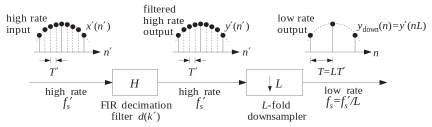
\includegraphics[width = 0.75\textwidth]{pic/dicimation.pdf}
		\begin{itemize}
		  \item Das schnell abgetastete Signal $x'(n')$ mit einem\\ digitalen Dezimierungsfilter auf das Nyquistband der\\ tiefen Abtastfrequenz $[-f_s/2,f_s/2]$ begrenzen.\\[-1.35cm]
		  \hspace*{10.2cm}\fcolorbox{CadetRed}{white}{$y'(n') = \mysum{k'}{\textcolor{white}{ds}}{h(k')\,x'(n'-k')}$}\\[-0.1cm]
		  \item Das bandbegrenzte Signal $y'(n')$ um den Faktor $L$ downsamplen, d.h. nur jedes $L$-te Sample behalten.\\[0.2cm]
		  \fcolorbox{CadetRed}{white}{$y_{down}(n) = y'(n')\big|_{n'=nL} = y'(nL)$}\\[-0.45cm]
		  \item Es resultiert ein Signal $y_{down}(n)$ welches eine tiefere Taktrate hat.$\qquad$
		  \fcolorbox{CadetRed}{white}{$f_s = \dfrac{f_s'}{L}\qquad\Leftrightarrow\qquad T = T'\cdot L$}\\[-0.4cm]
		\end{itemize}
		
	\subsection{Schritte im Frequenzbereich}
		\begin{itemize}
		  \item Spektrum $X'(f)$ des schnell abgetasteten Signal $x'(n')$,\\ welches mit dem Dezimierungsfilter $D(f)$ auf\\ das Nyquistband der tiefen Ab-\\ tastfrequenz $[-f_s/2,f_s/2]$\\ begrenzt wird.\\[-2.3cm]
		  \begin{minipage}{0.3\textwidth}$ $\end{minipage}
		  \begin{minipage}{0.7\textwidth}
			\hspace*{-1.36cm}\begin{tikzpicture}[>=latex, scale=0.9]
				\draw[->][line width=0.75](0,-0.2)node[below]{\small$0$}--(0,2.4)node[right]{\small$X'(f)$};
				\draw[->][line width=0.75](-6,0)--(6,0)node[below]{\small$f$};

				\draw[CadetRed, line width=1](-1.2*4,0)++(-1.2*2.5,0)++({(1.2*2+0.2)*0.7},{(1.3)*0.7})--++({(1.2*2+0.2)*0.3},{(1.3)*0.3})--node[above]{}++(0.8,0)--++(1.2*2+0.2,-1.3);
				\draw[CadetRed, line width=1](1.2*4,0)++(-1.2*2.5,0)--++(1.2*2+0.2,1.3)--node[above]{}++(0.8,0)--++(1.2*2*0.3+0.2*0.3,-1.3*0.3);
				\draw[blueT, line width=1](0,0)++(-1.2*2.5,0)--++(1.2*2+0.2,1.3)--node[above left,yshift=2pt]{\small $f_s'\,X_a(f)$}node[above right,yshift=2pt,gray]{\small $D(f)$}++(0.8,0)--++(1.2*2+0.2,-1.3);


				\draw[gray, line width=1.25](-1.2*4.5-0.3,0.1)--++(0.3,0)--++(0,1.3)--++(1.2,0)--++(0,-1.3)--++(1.2*3,0)--++(0,1.3)--++(1.2,0)--++(0,-1.3)--++(1.2*3,0)--++(0,1.3)--++(1.2,0)--++(0,-1.3)--++(0.3,0);

				\draw[line width=2, blueT](-0.6*4,0)--(0.6*4,-0);
				\draw[line width=0.75, blueT](-0.6*4,0.2)--(-0.6*4,-1.25);
				\draw[line width=0.75, blueT](0.6*4,0.2)--(0.6*4,-1.25);
				\draw[line width=0.75, blueT,<->](-0.6*4,-1.1)--node[fill=white]{\footnotesize Nyquistintervall}(0.6*4,-1.1);

			% 		\draw[line width=0.75](1.2*0.5,0.2)--(1.2*0.5,-0.2)node[below]{\small$f_s'/8$};
			% 		\draw[line width=0.75](-1.2*0.5,0.2)--(-1.2*0.5,-0.2)node[below]{\small$-f_s'/8\;\;\;\;$};		
				\draw[line width=0.75](1.2,0.2)--(1.2,-0.2)node[below]{\small$f_s'/L$};
				\draw[line width=0.75](-1.2,0.2)--(-1.2,-0.2)node[below]{\small$-f_s'/L$};
				\draw[line width=0.75](2*1.2,0.2)--(2*1.2,-0.2)node[below,fill=white]{\small$f_s'/2$};
				\draw[line width=0.75](-2*1.2,0.2)--(-2*1.2,-0.2)node[below,fill=white]{\small$-f_s'/2$};
				\draw[line width=0.75](3*1.2,0.2)--(3*1.2,-0.2)node[below=5pt]{\small$\dots$};
				\draw[line width=0.75](-3*1.2,0.2)--(-3*1.2,-0.2)node[below=5pt]{\small$ \dots$};
				\draw[line width=0.75](4*1.2,0.2)--(4*1.2,-0.2)node[below]{\small$f_s'$};
				\draw[line width=0.75](-4*1.2,0.2)--(-4*1.2,-0.2)node[below]{\small$-f_s'$};

				\begin{scope}[shift={(6,0)}]
					\draw[CadetRed, line width=1,fill](0,0.65)circle(1pt);
					\draw[CadetRed, line width=1,fill](0.25,0.65)circle(1pt);
					\draw[CadetRed, line width=1,fill](-0.25,0.65)circle(1pt);
				\end{scope}
				\begin{scope}[shift={(-6,0)}]
					\draw[CadetRed, line width=1,fill](0,0.65)circle(1pt);
					\draw[CadetRed, line width=1,fill](0.25,0.65)circle(1pt);
					\draw[CadetRed, line width=1,fill](-0.25,0.65)circle(1pt);
				\end{scope}
			\end{tikzpicture}
		  \end{minipage}\\[-0.0cm]
		  \item Spektrum $Y'(f)$ des gefilterten, schnell abgetasteten\\ Ausgangssignal $y'(n')$\\[-1.25cm]
		  \begin{minipage}{0.3\textwidth}$ $\end{minipage}
		  \begin{minipage}{0.7\textwidth}
			\begin{tikzpicture}[>=latex, scale=0.9]
				\draw[->][line width=0.75](0,-0.2)node[below]{\small$0$}--(0,2.2)node[right]{\small$Y'(f)$};
				\draw[->][line width=0.75](-6,0)--(6,0)node[below]{\small$f$};

				\foreach \i in {-4,0,4}
				{
					\draw[CadetRed, line width=1](1.2*\i,0)++(-0.6,0)--++(0,{1.3*(1-0.2/(1.2*2+0.2))})--++({(1.2*2+0.2)*0.2/(1.2*2+0.2)},{1.3*0.2/(1.2*2+0.2)})--++(0.8,0)--++({(1.2*2+0.2)*0.2/(1.2*2+0.2)},{-1.3*0.2/(1.2*2+0.2)})--++(0,{-1.3*(1-0.2/(1.2*2+0.2))});
				}

				\draw[blueT, line width=1](0,0)++(-0.6,0)--++(0,{1.3*(1-0.2/(1.2*2+0.2))})--++({(1.2*2+0.2)*0.2/(1.2*2+0.2)},{1.3*0.2/(1.2*2+0.2)})--node[above left,yshift=-0pt]{\small $ $}++(0.8,0)--++({(1.2*2+0.2)*0.2/(1.2*2+0.2)},{-1.3*0.2/(1.2*2+0.2)})--++(0,{-1.3*(1-0.2/(1.2*2+0.2))});

			% 	\draw[gray, line width=1.25](-1.2*4.5-0.3,0.1)--++(0.3,0)--++(0,1.3)--++(1.2,0)--++(0,-1.3)--++(1.2*3,0)--++(0,1.3)--++(1.2,0)--++(0,-1.3)--++(1.2*3,0)--++(0,1.3)--++(1.2,0)--++(0,-1.3)--++(0.3,0);

				\draw[line width=2, blueT](-0.6*4,0)--(0.6*4,-0);
				\draw[line width=0.75, blueT](-0.6*4,0.2)--(-0.6*4,-1.25);
				\draw[line width=0.75, blueT](0.6*4,0.2)--(0.6*4,-1.25);
				\draw[line width=0.75, blueT,<->](-0.6*4,-1.1)--node[fill=white]{\footnotesize Nyquistintervall}(0.6*4,-1.1);

			% 		\draw[line width=0.75](1.2*0.5,0.2)--(1.2*0.5,-0.2)node[below]{\small$f_s'/8$};
			% 		\draw[line width=0.75](-1.2*0.5,0.2)--(-1.2*0.5,-0.2)node[below]{\small$-f_s'/8\;\;\;\;$};		
				\draw[line width=0.75](1.2,0.2)--(1.2,-0.2)node[below]{\small$f_s'/L$};
				\draw[line width=0.75](-1.2,0.2)--(-1.2,-0.2)node[below]{\small$-f_s'/L$};
				\draw[line width=0.75](2*1.2,0.2)--(2*1.2,-0.2)node[below,fill=white]{\small$f_s'/2$};
				\draw[line width=0.75](-2*1.2,0.2)--(-2*1.2,-0.2)node[below,fill=white]{\small$-f_s'/2$};
				\draw[line width=0.75](3*1.2,0.2)--(3*1.2,-0.2)node[below=5pt]{\small$\dots$};
				\draw[line width=0.75](-3*1.2,0.2)--(-3*1.2,-0.2)node[below=5pt]{\small$ \dots$};
				\draw[line width=0.75](4*1.2,0.2)--(4*1.2,-0.2)node[below]{\small$f_s'$};
				\draw[line width=0.75](-4*1.2,0.2)--(-4*1.2,-0.2)node[below]{\small$-f_s'$};

				\begin{scope}[shift={(6,0)}]
					\draw[CadetRed, line width=1,fill](0,0.65)circle(1pt);
					\draw[CadetRed, line width=1,fill](0.25,0.65)circle(1pt);
					\draw[CadetRed, line width=1,fill](-0.25,0.65)circle(1pt);
				\end{scope}
				\begin{scope}[shift={(-6,0)}]
					\draw[CadetRed, line width=1,fill](0,0.65)circle(1pt);
					\draw[CadetRed, line width=1,fill](0.25,0.65)circle(1pt);
					\draw[CadetRed, line width=1,fill](-0.25,0.65)circle(1pt);
				\end{scope}
			\end{tikzpicture}
		  \end{minipage}\\[-0.4cm]
		  \item Durch das Downsamplen um den Faktor $L$ werden\\ die Teil-Spektrum $Y'(f)$ näher zusammen-\\ geschoben bzw. $L$-mal periodisch\\ widerhohlt.\\[1cm]
		  $\;\Rightarrow\quad$\fcolorbox{CadetRed}{white}{$Y_{down}(f) = \dfrac{1}{L}\mysum{m=0}{L-1}{Y'(f-mf_s)}$}\\[-3.9cm]
		  \begin{minipage}{0.3\textwidth}$ $\end{minipage}
		  \begin{minipage}{0.7\textwidth}
			\begin{tikzpicture}[>=latex, scale=0.9]
				\draw[->][line width=0.75](0,-0.2)node[below]{\small$0$}--(0,2.2)node[right]{\small$Y_{down}(f)$};
				\draw[->][line width=0.75](-6,0)--(6,0)node[below]{\small$f$};

				\draw[line width=0.75](1.2,0.2)--(1.2,-0.2)node[below]{\small$f_s$};
				\draw[line width=0.75](-1.2,0.2)--(-1.2,-0.2)node[below]{\small$-f_s$};
				\draw[line width=0.75](2*1.2,0.2)--(2*1.2,-0.2)node[below]{\small$2f_s$};
				\draw[line width=0.75](-2*1.2,0.2)--(-2*1.2,-0.2)node[below]{\small$-2f_s$};
				\draw[line width=0.75](3*1.2,0.2)--(3*1.2,-0.2)node[below=5pt]{\small$\dots$};
				\draw[line width=0.75](-3*1.2,0.2)--(-3*1.2,-0.2)node[below=5pt]{\small$\dots$};
				\draw[line width=0.75](4*1.2,0.2)--(4*1.2,-0.2)node[below]{\small$Lf_s$};
				\draw[line width=0.75](-4*1.2,0.2)--(-4*1.2,-0.2)node[below]{\small$-Lf_s$};
				

				\foreach \i in {-4,...,4}
				{
					\draw[CadetRed, line width=1](1.2*\i,0)++(-0.6,0)--++(0,{1.3*(1-0.2/(1.2*2+0.2))})--++({(1.2*2+0.2)*0.2/(1.2*2+0.2)},{1.3*0.2/(1.2*2+0.2)})--++(0.8,0)--++({(1.2*2+0.2)*0.2/(1.2*2+0.2)},{-1.3*0.2/(1.2*2+0.2)})--++(0,{-1.3*(1-0.2/(1.2*2+0.2))});
				}
				\draw[blueT, line width=1](0,0)++(-0.6,0)--++(0,{1.3*(1-0.2/(1.2*2+0.2))})--++({(1.2*2+0.2)*0.2/(1.2*2+0.2)},{1.3*0.2/(1.2*2+0.2)})--node[above left,yshift=-2pt]{\small $Y'(0)/L$}++(0.8,0)--++({(1.2*2+0.2)*0.2/(1.2*2+0.2)},{-1.3*0.2/(1.2*2+0.2)})--++(0,{-1.3*(1-0.2/(1.2*2+0.2))});

				\draw[line width=2, blueT](-0.6,0)--(0.6,-0);
				\draw[line width=0.75, blueT](-0.6,0.2)--(-0.6,-0.9);
				\draw[line width=0.75, blueT](0.6,0.2)--(0.6,-0.9);
				\draw[line width=0.75, blueT,<->](-0.6,-0.8)--node[below]{\footnotesize Nyquistintervall}(0.6,-0.8);


				\begin{scope}[shift={(6,0)}]
					\draw[CadetRed, line width=1,fill](0,0.65)circle(1pt);
					\draw[CadetRed, line width=1,fill](0.25,0.65)circle(1pt);
					\draw[CadetRed, line width=1,fill](-0.25,0.65)circle(1pt);
				\end{scope}
				\begin{scope}[shift={(-6,0)}]
					\draw[CadetRed, line width=1,fill](0,0.65)circle(1pt);
					\draw[CadetRed, line width=1,fill](0.25,0.65)circle(1pt);
					\draw[CadetRed, line width=1,fill](-0.25,0.65)circle(1pt);
				\end{scope}
			\end{tikzpicture}
		  \end{minipage}
		\end{itemize}
\newpage
		
		
	\subsection{Tiefpass - Dezimierungsfilter}
		\begin{itemize}
		 \item Das ideale Dezimierungsfilter ist ein idealer Tiefpass und fast identisch mit dem Interpolationsfilter.\\[0.2cm]
		 \begin{tabular}{lc|cl}
		  Frequenzgang: &&& Impulsantwort:\\[0.05cm]
		  \fcolorbox{CadetRed}{white}{$D(\omega') =$ \small$\begin{cases}1, & -\pi/L\leq \omega'\leq \pi/L\\ 0,&\text{sonst}\end{cases}$}&&&\fcolorbox{CadetRed}{white}{$d(k') = \dfrac{1}{2\pi}\myint{-\pi}{\pi}{D(\omega')\,\e^{j\omega'k'}}{\omega'} = \dfrac{\sin(\pi k'/L)}{\pi k'}$}\\[0.6cm]
		  Grenzfrequenz:&&& \\[0.05cm]
		  \fcolorbox{CadetRed}{white}{$f_c = \dfrac{f_s}{2}=\dfrac{f_s'}{2\,L}$}$\qquad$\fcolorbox{CadetRed}{white}{$\omega_c' = \dfrac{2\pi f_c}{f_s'}=\dfrac{\pi}{L}$} &&& \\[0.45cm]
		  Samplingfrequenz:&&&\\[0.05cm]
		  \fcolorbox{CadetRed}{white}{$f_s' = L\, f_s$} &&&\\
		 \end{tabular}\\[-3cm]
		 \hspace*{7.4cm}% 
% (c) Copyright 2016 Tabea Mendez
% 
% This source is free: you can redistribute it and/or modify
% it under the terms of the GNU General Public License as published by
% the Free Software Foundation, either version 3 of the License, or
% (at your option) any later version.
% 
% This source is distributed in the hope that it will be useful,
% but WITHOUT ANY WARRANTY; without even the implied warranty of
% MERCHANTABILITY or FITNESS FOR A PARTICULAR PURPOSE.  See the
% GNU General Public License for more details.
% 
% You should have received a copy of the GNU General Public License
% along with this source.  If not, see <http://www.gnu.org/licenses/>.
%
%%%%%%%%%%%%%%%%%%%%%%%%%%%%%%%%%%%%%%%%%%%%%%%%%%%%%%%%%%%%%%%%%%%%%%%%%%%%%%
\begin{tikzpicture}[>=latex, scale=0.9]
      \draw[->][line width=0.75](0,-0.2)node[below]{\small$0$}--(0,2.2)node[right]{$D(\omega')$};
      \draw[->][line width=0.75](-5.5,0)--(5.6,0)node[below]{$\omega'$};

% 			\draw[CadetRed, line width=1.5](-1.2*4.5-0.3,0)--++(0.3,0)--++(0,1.3)--++(1.2,0)--++(0,-1.3)--++(1.2*3,0)--++(0,1.3)--node[above left]{$L$}++(1.2,0)--++(0,-1.3)--++(1.2*3,0)--++(0,1.3)--++(1.2,0)--++(0,-1.3)--++(0.3,0);

      \draw[CadetRed, line width=1.5](-1*4.5-0.3-1.5*0.2,0)--++(0.3,0)--++(0,1.3)--++(1.2,0)--++(0,-1.3)--++(1*3,0)--++(0,1.3)--node[above left]{$1$}++(1.2,0)--++(0,-1.3)--++(1*3,0)--++(0,1.3)--++(1.2,0)--++(0,-1.3)--++(0.3,0);


% 		\draw[line width=2, blueT](-0.6*4,0)--(0.6*4,-0);
      \draw[line width=0.75, blueT](-0.6-0.5*3,0.2)--(-0.6-0.5*3,-1.25);
      \draw[line width=0.75, blueT](0.6+0.5*3,0.2)--(0.6+0.5*3,-1.25);
      \draw[line width=0.75, blueT,<->](-0.6-0.5*3,-1.1)--node[fill=white]{\footnotesize Nyquistintervall}(0.6+0.5*3,-1.1);

      \draw[line width=0.75](1.2*0.5,0.2)--(1.2*0.5,-0.2)node[below]{$\;\;\pi$\footnotesize$/L$};
      \draw[line width=0.75](-1.2*0.5,0.2)--(-1.2*0.5,-0.2)node[below]{-$\pi$\footnotesize$/L\;\;\;$};		
      \draw[line width=0.75](0.6+0.5*3,0.2)--(0.6+0.5*3,-0.2)node[below,fill=white]{ $\pi$};
      \draw[line width=0.75](-0.6-0.5*3,0.2)--(-0.6-0.5*3,-0.2)node[below,fill=white]{-$\pi$};
      \draw[line width=0.75](1.2+0.5*6,0.2)--(1.2+0.5*6,-0.2)node[below]{ $2\pi$};
      \draw[line width=0.75](-1.2-0.5*6,0.2)--(-1.2-0.5*6,-0.2)node[below]{ -$2\pi$};

      \begin{scope}[shift={(5.5,0)}]
	      \draw[CadetRed, line width=1,fill](0,0.65)circle(1pt);
	      \draw[CadetRed, line width=1,fill](0.25,0.65)circle(1pt);
	      \draw[CadetRed, line width=1,fill](-0.25,0.65)circle(1pt);
      \end{scope}
      \begin{scope}[shift={(-5.5,0)}]
	      \draw[CadetRed, line width=1,fill](0,0.65)circle(1pt);
	      \draw[CadetRed, line width=1,fill](0.25,0.65)circle(1pt);
	      \draw[CadetRed, line width=1,fill](-0.25,0.65)circle(1pt);
      \end{scope}
\end{tikzpicture}\\[-0.6cm]
		 \item Durch das abschneiden der Impulsantwort $d(k')$ des Tiefpasses ein bei $\pm ML$ ergibt sich ein akausales FIR-Filter. Dieses FIR-Filter läuft auf der hohen Abtastfrequenz $f_s'$.\\[0.2cm]
		 \hspace*{1cm}Akausales FIR-Filter:$\qquad$\fcolorbox{CadetRed}{white}{$y_{down}(n) = y'(nL) = \mysum{k'=-ML}{ML}{d(k')\,x'(nL-k')}$}\\[-0.1cm]
		 \item Der Tiefpass kann kausal gemacht werden, indem er um $ML$ Samples verzögert wird und eventuell noch mit einem Fenster $w(n')$ Multipliziert wird.\\[0.2cm]
		 \hspace*{1cm}Kausales FIR-Filter: $\qquad$\fcolorbox{CadetRed}{white}{$h(n') = w(n')\,d(n'-ML)$}$\qquad n' = 0,1,...,N-1$\\[0.2cm]
		 \hspace*{4.17cm}$\Rightarrow\qquad$\fcolorbox{CadetRed}{white}{$y_{down}(n) = y'(nL) = \mysum{k'=0}{N-1}{w(k')\,d(k'-ML)\,x'(nL-k')}$}$\quad$\fcolorbox{black}{white}{$N = 2ML+1$}\\[-0.1cm]
		 \item Da nur jedes $L$-te Sample verwendet wird, ist es nicht sinnvoll jedes Sample der hohen Abtastfrequenz $y'(n')$ zu berechnen. Damit nur die Samples $y'(nL)$ berechnet werden, muss das Eingangssignal $x'(n')$ vor jedem Filterkoeffizienten downgesampelt werden, womit sich der Rechenaufwand stark reduziert.\\[0.2cm]
		 \hspace*{0.83cm}\begin{tabular}{ll}
		  Normales-Filter: & \fcolorbox{black}{white}{$2ML^2$ - Multiplikationen pro Sample}\\[0.2cm]
		  Downgesampeltes-Filter:& \fcolorbox{black}{white}{$2ML$ - Multiplikationen pro Sample}\\
		 \end{tabular}\\[-0.1cm]
		 \item Normales-Filter / Downgesampeltes-Filter\\[0.2cm]
			\begin{minipage}{0.5\textwidth}
			% 
% (c) Copyright 2016 Tabea Mendez
% 
% This source is free: you can redistribute it and/or modify
% it under the terms of the GNU General Public License as published by
% the Free Software Foundation, either version 3 of the License, or
% (at your option) any later version.
% 
% This source is distributed in the hope that it will be useful,
% but WITHOUT ANY WARRANTY; without even the implied warranty of
% MERCHANTABILITY or FITNESS FOR A PARTICULAR PURPOSE.  See the
% GNU General Public License for more details.
% 
% You should have received a copy of the GNU General Public License
% along with this source.  If not, see <http://www.gnu.org/licenses/>.
%
%%%%%%%%%%%%%%%%%%%%%%%%%%%%%%%%%%%%%%%%%%%%%%%%%%%%%%%%%%%%%%%%%%%%%%%%%%%%%%
\begin{tikzpicture}[>=latex', scale=1.1]
\def\s{0.3};
\def\l{1.4};
\def\dh{0.8};
\def\dv{0.6};

	% Erste Abteilung	
	\begin{scope}[yshift=0.5cm]
		\coordinate (m) at (-\s-\l,0);
		\draw[line width=1](-\l,0)--node[above]{\footnotesize$x'(n')$}node[below]{\footnotesize$f_s'$}++(\l,0);


		\coordinate (np) at (0,0);
		\draw[line width=1,->](np)--++(\dh,0);
		\draw[line width=1,->](np)--++(0,-2*\dv-0.5)--++(\dh,0)node[xshift=-1.8cm]{\Large$\ast$}node[xshift=-1.8cm,yshift=1.1cm]{\Large$\ast$};

		\coordinate (m) at (0,-\dv-0.5);
		\draw[line width=1,fill=white](m)++(-\s,-\s)--++(2*\s,0)--++(0,2*\s)--++(-2*\s,0)--cycle node at(m)[xshift=0pt]{\small$\zeta^{\text{-}1}$};

		\coordinate (m) at (\dh,0);
		\draw[line width=1,fill=white](m)--++(0,1.1*\s)--++(2.1*\s,-1.1*\s)--++(-2.1*\s,-1.1*\s)--cyclenode at(m)[right, xshift=5pt,yshift=11pt]{\small$h_{0}$};
		\coordinate (m) at (\dh,-2*\dv-0.5);
		\draw[line width=1,fill=white](m)--++(0,1.1*\s)--++(2.1*\s,-1.1*\s)--++(-2.1*\s,-1.1*\s)--cyclenode at(m)[right, xshift=5pt,yshift=11pt]{\small$h_{1}$};

		\draw[line width=1](np)++(\dh+2*\s,0)--(2.5*\dh+2*\s,0);
		\draw[line width=1](np)++(\dh+2*\s,-2*\dv-0.5)--++(0.9*\dh,0)--(2.5*\dh+2*\s,0);

		\draw[line width=1,->](np)++(2.5*\dh+2*\s,0)--node[above]{\footnotesize$y'(n')$}node[below]{\footnotesize$f_s'$}++(1.2*\l,0);

		\draw[line width=1,->](2.5*\dh+4*\s+1.2*\l,0)--node[above]{\footnotesize$y_{down}(n)$}node[below]{\footnotesize$f_s$}++(1.2*\l,0);
		\coordinate (m) at (2.5*\dh+3*\s+1.2*\l,0);
		\draw[line width=1,fill=white](m)++(-\s,-\s)--++(2*\s,0)--++(0,2*\s)--++(-2*\s,0)--cycle node at(m)[xshift=-3.5pt]{\small$\downarrow$};
		\node at(m)[xshift=2.5pt]{\small$L$};
	
		\foreach \i in {0,1,2,3}
		{
			\coordinate (m) at (2.5*\dh+3*\s+1.2*\l,-\i*1.7);
% 			\node at(m)[xshift=-1.25cm,yshift=-1cm,CadetRed]{\Large$\bm\ast$};
			\node at(m)[xshift=-1.25cm,yshift=-1.4cm]{\Large$\ast$};
			\node at(m)[xshift=-1.25cm,yshift=-1.8cm]{$\vdots$};
			\node at(m)[xshift=-1.25cm,yshift=-2.45cm]{\Large$\ast$};
		}
		\node at(m)[xshift=-1.25cm,yshift=-2.45cm,fill,white]{\Large$\ast$};

			\coordinate (m) at (2.5*\dh+3*\s+1.2*\l,-0*1.7);
			\node at(m)[xshift=-1.15cm,yshift=-1cm,CadetRed]{\Large$\bm\ast_{\text{\footnotesize$0$}}$};
			\coordinate (m) at (2.5*\dh+3*\s+1.2*\l,-1*1.7);
			\node at(m)[xshift=-1.12cm,yshift=-1cm,CadetRed]{\Large$\bm\ast_{\text{\footnotesize$L$}}$};
			\coordinate (m) at (2.5*\dh+3*\s+1.2*\l,-2*1.7);
			\node at(m)[xshift=-1.04cm,yshift=-1cm,CadetRed]{\Large$\bm\ast_{\text{\footnotesize$2L$}}$};
			\coordinate (m) at (2.5*\dh+3*\s+1.2*\l,-3*1.7);
			\node at(m)[xshift=-1.04cm,yshift=-1cm,CadetRed]{\Large$\bm\ast_{\text{\footnotesize$3L$}}$};

		\coordinate (m) at (2.5*\dh+3*\s+1.2*\l,-0*0.37);
		\node at(m)[xshift=1.35cm,yshift=-1cm,CadetRed]{\Large$\bm\ast_{\text{\footnotesize$0$}}$};
		\coordinate (m) at (2.5*\dh+3*\s+1.2*\l,-1*0.37);
		\node at(m)[xshift=1.38cm,yshift=-1cm,CadetRed]{\Large$\bm\ast_{\text{\footnotesize$L$}}$};
		\coordinate (m) at (2.5*\dh+3*\s+1.2*\l,-2*0.37);
		\node at(m)[xshift=1.465cm,yshift=-1cm,CadetRed]{\Large$\bm\ast_{\text{\footnotesize$2L$}}$};
		\coordinate (m) at (2.5*\dh+3*\s+1.2*\l,-3*0.37);
		\node at(m)[xshift=1.46cm,yshift=-1cm,CadetRed]{\Large$\bm\ast_{\text{\footnotesize$3L$}}$};
		\node at(m)[xshift=1.25cm,yshift=-1.4cm]{$\vdots$};

	\end{scope}

	% Zeite Abteilung
	\begin{scope}[yshift=-0.9cm]
		\coordinate (np) at (0,0);
		\draw[line width=1](np)++(0,-0.5*\dv)--++(0,{-(\dv-\s)});
		\draw[line width=1](np)++(0,-1.5*\dv)--++(0,-5*\dv);
		\draw[line width=1,->](np)++(0,-2.5*\dv)--++(\dh,0)node[xshift=-1.8cm]{\Large$\ast$};
		\draw[line width=1,->](np)++(0,-4.5*\dv)--++(\dh,0)node[xshift=-1.8cm]{\Large$\ast$};
		\draw[line width=1,->](np)++(0,-6.5*\dv)--++(\dh,0)node[xshift=-1.8cm]{\Large$\ast$};

		\coordinate (m) at (0,-1.5*\dv);
		\draw[line width=1,fill=white](m)++(-\s,-\s)--++(2*\s,0)--++(0,2*\s)--++(-2*\s,0)--cycle node at(m)[xshift=0pt]{\small$\zeta^{\text{-}1}$};
		\coordinate (m) at (0,-3.5*\dv);
		\draw[line width=1,fill=white](m)++(-\s,-\s)--++(2*\s,0)--++(0,2*\s)--++(-2*\s,0)--cycle node at(m)[xshift=0pt]{\small$\zeta^{\text{-}1}$};
		\coordinate (m) at (0,-5.5*\dv);
		\draw[line width=1,fill=white](m)++(-\s,-\s)--++(2*\s,0)--++(0,2*\s)--++(-2*\s,0)--cycle node at(m)[xshift=0pt]{\small$\zeta^{\text{-}1}$};

		\coordinate (m) at (\dh,-2.5*\dv);
		\draw[line width=1,fill=white](m)--++(0,1.1*\s)--++(2.1*\s,-1.1*\s)--++(-2.1*\s,-1.1*\s)--cyclenode at(m)[right, xshift=5pt,yshift=11pt]{\small$h_2$};
		\coordinate (m) at (\dh,-4.5*\dv);
		\draw[line width=1,fill=white](m)--++(0,1.1*\s)--++(2.1*\s,-1.1*\s)--++(-2.1*\s,-1.1*\s)--cyclenode at(m)[right, xshift=5pt,yshift=11pt]{\small$h_3$};
		\coordinate (m) at (\dh,-6.5*\dv);
		\draw[line width=1,fill=white](m)--++(0,1.1*\s)--++(2.1*\s,-1.1*\s)--++(-2.1*\s,-1.1*\s)--cyclenode at(m)[right, xshift=5pt,yshift=11pt]{\small$h_4$};

		\draw[line width=1](np)++(\dh+2*\s,-2.5*\dv)--++(0.8*\dh,0)--(2.5*\dh+2*\s,1.4);
		\draw[line width=1](np)++(\dh+2*\s,-4.5*\dv)--++(0.775*\dh,0)--(2.5*\dh+2*\s,1.4);
		\draw[line width=1](np)++(\dh+2*\s,-6.5*\dv)--++(0.8*\dh,0)--(2.5*\dh+2*\s,1.4);

	\end{scope}

	\begin{scope}[yshift=-5.1cm]
		\coordinate (np) at (0,0);
		\draw[line width=1,dashed, dash phase=-0pt, dash pattern=on 3.2pt off 3pt](np)++(0,0.5*\dv)--++(0,{-(2*\dv-\s)});
		\draw[line width=1,->](np)++(0,-1.5*\dv)--++(0,-1*\dv)--++(\dh,0)node[xshift=-1.8cm]{\Large$\ast$}node[xshift=-1.8cm,yshift=1.1cm]{\small$\vdots$};

		\coordinate (m) at (0,-1.5*\dv);
		\draw[line width=1,fill=white](m)++(-\s,-\s)--++(2*\s,0)--++(0,2*\s)--++(-2*\s,0)--cycle node at(m)[xshift=0pt]{\small$\zeta^{\text{-}1}$};


		\coordinate (m) at (\dh,-2.5*\dv);
		\draw[line width=1,fill=white](m)--++(0,1.1*\s)--++(2.1*\s,-1.1*\s)--++(-2.1*\s,-1.1*\s)--cyclenode at(m)[right, xshift=5pt,yshift=11pt]{\small$h_{2ML}$};

		\draw[line width=1](m)++(2*\s,0)--++(0.85*\dh,0)--(2.5*\dh+2*\s,5.6);


	\end{scope}


	% Addirer
	\draw[line width=1,white,fill](2.5*\dh+2*\s,0.5)circle(5.5pt)node[black]{\Large$\bigoplus$};


\end{tikzpicture}

			\end{minipage}
			\begin{minipage}{0.5\textwidth}
			% 
% (c) Copyright 2016 Tabea Mendez
% 
% This source is free: you can redistribute it and/or modify
% it under the terms of the GNU General Public License as published by
% the Free Software Foundation, either version 3 of the License, or
% (at your option) any later version.
% 
% This source is distributed in the hope that it will be useful,
% but WITHOUT ANY WARRANTY; without even the implied warranty of
% MERCHANTABILITY or FITNESS FOR A PARTICULAR PURPOSE.  See the
% GNU General Public License for more details.
% 
% You should have received a copy of the GNU General Public License
% along with this source.  If not, see <http://www.gnu.org/licenses/>.
%
%%%%%%%%%%%%%%%%%%%%%%%%%%%%%%%%%%%%%%%%%%%%%%%%%%%%%%%%%%%%%%%%%%%%%%%%%%%%%%
\begin{tikzpicture}[>=latex', scale=1.1]
\def\s{0.3};
\def\l{1.4};
\def\dh{0.8};
\def\dv{0.6};

	% Erste Abteilung	
	\begin{scope}[yshift=0.5cm]
		\coordinate (m) at (-\s-\l,0);
		\draw[line width=1](-\l,0)--node[above]{\footnotesize$x'(n')$}node[below]{\footnotesize$f_s'$}++(\l,0);


		\coordinate (np) at (0,0);
		\draw[line width=1,->](np)--++(\dh,0);
		\draw[line width=1,->](np)--++(0,-2*\dv-0.5)--++(\dh,0)node[xshift=-1.8cm]{\Large$\ast$}node[xshift=-1.8cm,yshift=1.1cm]{\Large$\ast$};

		\coordinate (m) at (0,-\dv-0.5);
		\draw[line width=1,fill=white](m)++(-\s,-\s)--++(2*\s,0)--++(0,2*\s)--++(-2*\s,0)--cycle node at(m)[xshift=0pt]{\small$\zeta^{\text{-}1}$};

		\coordinate (m) at (\dh+\s,0);
		\draw[line width=1,fill=white](m)++(-\s,-\s)--++(2*\s,0)--++(0,2*\s)--++(-2*\s,0)--cycle node at(m)[xshift=-3.5pt]{\small$\downarrow$};
		\node at(m)[xshift=2.5pt]{\small$L$};
		\draw[line width=1,->](m)++(\s,0)--node[below]{\footnotesize$f_s$}++(\dh,0);
		\draw[line width=1,fill=white](m)++(\dh+\s,0)--++(0,1.1*\s)--++(2.1*\s,-1.1*\s)--++(-2.1*\s,-1.1*\s)--cyclenode[above right, xshift=5pt,yshift=12pt]{\small$h_{0}$};
		\draw[line width=1](m)++(\dh+3*\s,0)--(3.5*\dh+4*\s,0);


		\coordinate (m) at (\dh+\s,-2*\dv-0.5);
		\draw[line width=1,fill=white](m)++(-\s,-\s)--++(2*\s,0)--++(0,2*\s)--++(-2*\s,0)--cycle node at(m)[xshift=-3.5pt]{\small$\downarrow$};
		\node at(m)[xshift=2.5pt]{\small$L$};
		\draw[line width=1,->](m)++(\s,0)--node[below]{\footnotesize$f_s$}++(\dh,0);
		\draw[line width=1,fill=white](m)++(\dh+\s,0)--++(0,1.1*\s)--++(2.1*\s,-1.1*\s)--++(-2.1*\s,-1.1*\s)--cyclenode[above right, xshift=5pt,yshift=12pt]{\small$h_{1}$};
		\draw[line width=1](m)++(\dh+3*\s,0)--++(0.725,0)--(3.5*\dh+4*\s,0);


		\draw[line width=1,->](np)++(3.5*\dh+4*\s,0)--node[above]{\footnotesize$y_{down}(n)$}node[below]{\footnotesize$f_s$}++(1.4*\l,0);


		\coordinate (m) at (2.5*\dh+3*\s+1.2*\l-0.8,-0*0.37);
		\node at(m)[xshift=1.35cm,yshift=-1cm,CadetRed]{\Large$\bm\ast_{\text{\footnotesize$0$}}$};
		\coordinate (m) at (2.5*\dh+3*\s+1.2*\l-0.8,-1*0.37);
		\node at(m)[xshift=1.38cm,yshift=-1cm,CadetRed]{\Large$\bm\ast_{\text{\footnotesize$L$}}$};
		\coordinate (m) at (2.5*\dh+3*\s+1.2*\l-0.8,-2*0.37);
		\node at(m)[xshift=1.465cm,yshift=-1cm,CadetRed]{\Large$\bm\ast_{\text{\footnotesize$2L$}}$};
		\coordinate (m) at (2.5*\dh+3*\s+1.2*\l-0.8,-3*0.37);
		\node at(m)[xshift=1.46cm,yshift=-1cm,CadetRed]{\Large$\bm\ast_{\text{\footnotesize$3L$}}$};
		\node at(m)[xshift=1.25cm,yshift=-1.4cm]{$\vdots$};

	\end{scope}

	% Zeite Abteilung
	\begin{scope}[yshift=-0.9cm]
		\coordinate (np) at (0,0);
		\draw[line width=1](np)++(0,-0.5*\dv)--++(0,{-(\dv-\s)});
		\draw[line width=1](np)++(0,-1.5*\dv)--++(0,-5*\dv);
		\draw[line width=1,->](np)++(0,-2.5*\dv)--++(\dh,0)node[xshift=-1.8cm]{\Large$\ast$};
		\draw[line width=1,->](np)++(0,-4.5*\dv)--++(\dh,0)node[xshift=-1.8cm]{\Large$\ast$};
		\draw[line width=1,->](np)++(0,-6.5*\dv)--++(\dh,0)node[xshift=-1.8cm]{\Large$\ast$};

		\coordinate (m) at (0,-1.5*\dv);
		\draw[line width=1,fill=white](m)++(-\s,-\s)--++(2*\s,0)--++(0,2*\s)--++(-2*\s,0)--cycle node at(m)[xshift=0pt]{\small$\zeta^{\text{-}1}$};
		\coordinate (m) at (0,-3.5*\dv);
		\draw[line width=1,fill=white](m)++(-\s,-\s)--++(2*\s,0)--++(0,2*\s)--++(-2*\s,0)--cycle node at(m)[xshift=0pt]{\small$\zeta^{\text{-}1}$};
		\coordinate (m) at (0,-5.5*\dv);
		\draw[line width=1,fill=white](m)++(-\s,-\s)--++(2*\s,0)--++(0,2*\s)--++(-2*\s,0)--cycle node at(m)[xshift=0pt]{\small$\zeta^{\text{-}1}$};

		\coordinate (m) at (\dh+\s,-2.5*\dv);
		\draw[line width=1,fill=white](m)++(-\s,-\s)--++(2*\s,0)--++(0,2*\s)--++(-2*\s,0)--cycle node at(m)[xshift=-3.5pt]{\small$\downarrow$};
		\node at(m)[xshift=2.5pt]{\small$L$};
		\draw[line width=1,->](m)++(\s,0)--node[below]{\footnotesize$f_s$}++(\dh,0);
		\draw[line width=1,fill=white](m)++(\dh+\s,0)--++(0,1.1*\s)--++(2.1*\s,-1.1*\s)--++(-2.1*\s,-1.1*\s)--cyclenode[above right, xshift=5pt,yshift=12pt]{\small$h_{2}$};
		\draw[line width=1](m)++(\dh+3*\s,0)--++(0.67,0)--(3.5*\dh+4*\s,0.9+0.5);

		\coordinate (m) at (\dh+\s,-4.5*\dv);
		\draw[line width=1,fill=white](m)++(-\s,-\s)--++(2*\s,0)--++(0,2*\s)--++(-2*\s,0)--cycle node at(m)[xshift=-3.5pt]{\small$\downarrow$};
		\node at(m)[xshift=2.5pt]{\small$L$};
		\draw[line width=1,->](m)++(\s,0)--node[below]{\footnotesize$f_s$}++(\dh,0);
		\draw[line width=1,fill=white](m)++(\dh+\s,0)--++(0,1.1*\s)--++(2.1*\s,-1.1*\s)--++(-2.1*\s,-1.1*\s)--cyclenode[above right, xshift=5pt,yshift=12pt]{\small$h_{3}$};
		\draw[line width=1](m)++(\dh+3*\s,0)--++((0.675,0)--(3.5*\dh+4*\s,0.9+0.5);

		\coordinate (m) at (\dh+\s,-6.5*\dv);
		\draw[line width=1,fill=white](m)++(-\s,-\s)--++(2*\s,0)--++(0,2*\s)--++(-2*\s,0)--cycle node at(m)[xshift=-3.5pt]{\small$\downarrow$};
		\node at(m)[xshift=2.5pt]{\small$L$};
		\draw[line width=1,->](m)++(\s,0)--node[below]{\footnotesize$f_s$}++(\dh,0);
		\draw[line width=1,fill=white](m)++(\dh+\s,0)--++(0,1.1*\s)--++(2.1*\s,-1.1*\s)--++(-2.1*\s,-1.1*\s)--cyclenode[above right, xshift=5pt,yshift=12pt]{\small$h_{4}$};
		\draw[line width=1](m)++(\dh+3*\s,0)--++(0.7,0)--(3.5*\dh+4*\s,0.9+0.5);

	\end{scope}

	\begin{scope}[yshift=-5.1cm]
		\coordinate (np) at (0,0);
		\draw[line width=1,dashed, dash phase=-0pt, dash pattern=on 3.2pt off 3pt](np)++(0,0.5*\dv)--++(0,{-(2*\dv-\s)});
		\draw[line width=1,->](np)++(0,-1.5*\dv)--++(0,-1*\dv)--++(\dh,0)node[xshift=-1.8cm]{\Large$\ast$}node[xshift=-1.8cm,yshift=1.1cm]{\small$\vdots$};

		\coordinate (m) at (0,-1.5*\dv);
		\draw[line width=1,fill=white](m)++(-\s,-\s)--++(2*\s,0)--++(0,2*\s)--++(-2*\s,0)--cycle node at(m)[xshift=0pt]{\small$\zeta^{\text{-}1}$};


		\coordinate (m) at (\dh+\s,-2.5*\dv);
		\draw[line width=1,fill=white](m)++(-\s,-\s)--++(2*\s,0)--++(0,2*\s)--++(-2*\s,0)--cycle node at(m)[xshift=-3.5pt]{\small$\downarrow$};
		\node at(m)[xshift=2.5pt]{\small$L$};
		\draw[line width=1,->](m)++(\s,0)--node[below]{\footnotesize$f_s$}++(\dh,0);
		\draw[line width=1,fill=white](m)++(\dh+\s,0)--++(0,1.1*\s)--++(2.1*\s,-1.1*\s)--++(-2.1*\s,-1.1*\s)--cyclenode[above right, xshift=5pt,yshift=12pt]{\small$h_{2ML}$};
		\draw[line width=1](m)++(\dh+3*\s,0)--++(0.7,0)--(3.5*\dh+4*\s,5.1+0.5);



	\end{scope}


	% Addirer
	\draw[line width=1,white,fill](3.5*\dh+4*\s,0.5)circle(5.5pt)node[black]{\Large$\bigoplus$};


\end{tikzpicture}

			\end{minipage}
		\end{itemize}

	\subsection{Einfaches Dezimierungsfilter}
		Ein sehr einfaches Dezimierungsfilter ist, $L$-schnelle Samples zu einem langsamen Sample zu mitteln.\\[0.1cm]
		\begin{tabular}{lc|cl}
			Übertragungsfunktion:&$\!\!\!$&$\!\!\!$& Ausgangssignal:\\[0.1cm]
			\fcolorbox{CadetRed}{white}{$H(\zeta) = \dfrac{1}{L}\big[1 + \zeta^{-1} + ... + \zeta^{-(L-1)}\big] = \dfrac{1}{L}\dfrac{1-\zeta^{-L}}{1-\zeta^{-1}}$}&$\!\!\!$&$\!\!\!$& \fcolorbox{CadetRed}{white}{$y_{down}(n) = \dfrac{x'(nL)+x'(nL-1)+...+x'(nL-(L-1))}{L}$}\\
		\end{tabular}

\section{Noise-Shaping Quantisierer}
		Die Idee von Noise-Shaping ist, das Quantisierungsrauschen umzuverteilen, sodass im Frequenzband $[-\frac{f_s}{2},\frac{f_s}{2}]$ des analogen Eingangssignal $x_a(t)$ bzw. des dezimierten und downgesampelten Signals $y_{down}(n)$ möglichst wenig Rauschleistung vorhanden ist.\\[0.2cm]
		\hspace*{0cm}$\quad\Rightarrow\quad$\fcolorbox{CadetRed}{white}{$\begin{array}{l}\text{Rauschleistung in hohe Frequenzen verschieben, wo keine Signalleistung mehr vorhanden ist,}\\ \text{damit das Rauschen anschliessend herausgefiltert werden kann.}\end{array}$}\\[0.3cm]
		Dies wird bspw. beim Delta-Sigma-Wandler gemacht, indem ein Feedback-Pfad eingeführt wird.\\[-0.6cm]
		\begin{itemize}
		 \item Differenz $\Delta$ zwischen analogem Eingangssignal und dem digitalisierten Signal wird aufsummiert $\Sigma$\\[-0.6cm]
		 \item Integrator (Summierer) kann ...\\
		 ... langsamen Signalen gut folgen$\quad\Rightarrow\quad$ kleiner Quantisierungsfeher.\\
		 ... schnellen Signalen schlecht folgen$\quad\Rightarrow\quad$ grosser Quantisierungsfeher.\\ [0.2cm]
		 $\quad\Rightarrow\quad$ \fcolorbox{CadetRed}{white}{Integrator muss Frequenzen des analogen Signals $[-f_s/2\leq f \leq f_s/2]$ gut folgen können!}\\[0.2cm]
		 \includegraphics[width = 0.6\textwidth]{pic/sigmaDelta.pdf}
		\end{itemize}

		\textbf{Stochastisches, lineares diskretes Modell}\\[-0.9cm]
		\begin{minipage}{0.5\textwidth}
			\includegraphics[width = \textwidth]{pic/sigmaDeltaModel.pdf}\\
		\end{minipage}
		\begin{minipage}{0.4\textwidth}
			$\quad$\begin{tikzpicture}[>=latex', scale=1.7]
				\draw[->][line width=0.75](0,-0.3)--(0,1.2)node[above right]{\footnotesize$S_{\varepsilon\varepsilon}(f)$}node[above]{\footnotesize / }node[above left, CadetRed]{\footnotesize$S_{ee}(f)$};
				\draw[->][line width=0.75](-2.5,0)--(2.7,0)node[below]{\footnotesize$f$};
				\draw[line width=1,CadetRed](-2.5,0)--(-2,0)--(-2,0.7)node[left]{\footnotesize$\dfrac{\sigma_e'^2}{f'_s}$}--(2,0.7)--(2,0)--(2.5,0);
				\draw[line width=0.5](-2,0.1)--(-2,-0.1)node[below=-1pt]{\footnotesize -$\dfrac{f'_s}{2}$};
				\draw[line width=0.5](2,0.1)--(2,-0.1)node[below=-1pt]{\footnotesize $\dfrac{f'_s}{2}$};

	% 			\draw[line width=0.01,gray,fill, opacity=0.5](-0.7,0)--(-0.7,0.7)--(0.7,0.7)--(0.7,0)--cyclenode at (0.25,0.4)[darkgray, opacity=1]{$ $};

	% 			\draw[line width=1,blueT](-2,0)--(-0.7,0)--(-0.7,0.7)node[above]{\footnotesize$\dfrac{\sigma_e^2}{f_s}$}--(0.7,0.7)--(0.7,0)--(2,0);
				\draw[line width=0.5,dashed](0.7,-0.1)--(0.7,0.7);
				\draw[line width=0.5,dashed](-0.7,-0.1)--(-0.7,0.7);

				\draw[line width=0.5](-0.7,0.1)--(-0.7,-0.1)node[below]{\footnotesize -$\dfrac{f_s}{2}$};
				\draw[line width=0.5](0.7,0.1)--(0.7,-0.1)node[below]{\footnotesize $\dfrac{f_s}{2}$};

				\draw[CadetRed, line width=0.5, fill](2.3,0.3)circle(0.03);
				\draw[CadetRed, line width=0.5, fill](2.45,0.3)circle(0.03);
				\draw[CadetRed, line width=0.5, fill](2.6,0.3)circle(0.03);
				\draw[CadetRed, line width=0.5, fill](-2.3,0.3)circle(0.03);
				\draw[CadetRed, line width=0.5, fill](-2.45,0.3)circle(0.03);
				\draw[CadetRed, line width=0.5, fill](-2.6,0.3)circle(0.03);

				\draw[black, smooth,samples=100,domain=-2:2, line width=1](-2,0.7)--plot (\x,{0.25*abs(2*sin(\x*pi/4.5*180/pi))^2})node[above] {\footnotesize$\dfrac{\sigma_e'^2}{f_s'}|H_{NS}(f)|^2$}--(2,0.7);
				\draw[black, smooth,samples=100,domain=-0.7:0.7, line width=1, fill, opacity=0.5](-0.7,0)--plot (\x,{0.25*abs(2*sin(\x*pi/4.5*180/pi))^2})node[right] {$ $}--(0.7,0);
				\draw[black,line width=1](0.625,0.075)--++(0.2,0.05)node[right,yshift=3pt] {$\sigma_{e}^2$};
			\end{tikzpicture}\\[1.1cm]
		\end{minipage}\\[-1.7cm]
		\begin{itemize}
		 \item Übertragungsfunktion des Summierers:$\qquad$\fcolorbox{CadetRed}{white}{$H(\zeta) = \dfrac{\zeta^{-1}}{1-\zeta^{-1}}$}\\[-0.2cm]
		 \item Ausgangssignale des Delta-Sigma-Wandlers:\\[-0.55cm]
		 \hspace*{0.5cm}$H(\zeta)(X'(\zeta)-Y'(\zeta))+E'(\zeta) = Y'(\zeta)\qquad\Rightarrow\qquad Y'(\zeta) =\overbrace{\dfrac{H(\zeta)}{1+H(\zeta)}}^{\zeta^{-1}}X'(\zeta)+ \overbrace{\dfrac{1}{1+H(\zeta)}}^{1-\zeta^{-1}}E'(\zeta) $\\[0.25cm]
		 \hspace*{0.5cm}$\Rightarrow\qquad$\fcolorbox{CadetRed}{white}{$ Y'(\zeta) =H_X(\zeta)\,X'(\zeta)+ H_{NS}(\zeta)\,E'(\zeta) $}$\qquad$mit$\qquad$\fcolorbox{CadetRed}{white}{$H_X(\zeta) = \zeta^{-1},\qquad H_{NS}(\zeta)= 1-\zeta^{-1}$}\\[0.25cm]
		 \hspace*{0.5cm}$\Rightarrow\qquad$\fcolorbox{CadetRed}{white}{$ y'(n') =x'(n'-1)+ \varepsilon(n')$}$\qquad$mit$\qquad$\fcolorbox{CadetRed}{white}{$\varepsilon(n') = e(n') -e(n'-1)\quad\Leftrightarrow\quad \text{\LARGE$\varepsilon$}(\zeta) = (1-\zeta^{-1})E(\zeta)$}\\[-0.3cm]
		 \item Leistung des Quantisierungsrauschen nach dem Noise-Shaping:\\[0.2cm]
		 \fcolorbox{CadetRed}{white}{$\sigma_e^2 = \dfrac{\sigma_e'^2}{f'_s}\myint{-f_s/2}{f_s/2}{|H_{NS}(f)|^2}{f}$}$\qquad$\fcolorbox{CadetRed}{white}{$|H_{NS}(f)|^2 = \left|2\,\sin\left(\dfrac{\pi f}{f_s'}\right)\right|^{2p}\quad$ für $-\dfrac{f_s'}{2}\leq f\leq \dfrac{f_s'}{2}$}$\;\;\begin{array}{ll}p:&\text{Ordnung des}\\&\text{Noise-Shapers}\end{array}$\\[0cm]
		 \item Bitgewinn durch das Noise-Shaping\\ (Herleitung siehe Kapitel \ref{NoiseShapingHerleitung})\\[-1.1cm]
		 \hspace*{7cm}\fcolorbox{CadetRed}{white}{$\Delta B = (p+0.5)\,\log_2(L)-0.5\,\log_2\left(\dfrac{\pi^{2p}}{2p+1}\right)$}
		\end{itemize}
\newpage
		\subsection{Noise-Shaping Requantisierer}
			Die Idee des Noise-Shaping kann auch bei Digital-Analog-Wandlern angewendet werden. Das Ziel hierbei ist mit weniger Bits $B'<B$ des DAC ein qualitativ gleichwertiges analoges Ausgangssignal $x_a(t)$ zu erzeugen.\\[0.2cm]
			Dazu wird folgendes gemacht.\\[-0.5cm]
			\begin{itemize}
			 \item Der Quantisierer teilt das $B$-bit-Wort lange in zwei Wörter auf:\\
			 $-$ $w_{MSB}$: $\;B'$ - most-significant-Bits werden zum DAC weitergeleitet.\\
			 $-$ $w_{LSB}$: $\;(B-B')$ - least-significant-Bits (Rausch-Bits) werden durch das Loop-Filter geschickt.
			 \item Die Rausch-Bits (least-significant-Bits) werden vom Eingangssignal abgezogen, wodurch sie Hochpass gefiltert werden.\\[0.2cm]
			 $\quad\Rightarrow\quad$\fcolorbox{CadetRed}{white}{Das Rauschen wird Hochpass gefiltert und dadurch im tieffrequenten Band reduziert.}\\[0.2cm]
			 \includegraphics[width = 0.65\textwidth]{pic/requantModel1.pdf}
			\end{itemize}

			\textbf{Stochastisches, lineares diskretes Modell}\\[0.1cm]
			\includegraphics[width = 0.55\textwidth]{pic/requantModel2.pdf}\\[-0.2cm]
			\begin{itemize}
			\item Ausgangssignale des Noise-Shaping Requantisierers:\\[0.2cm]
			\hspace*{0.5cm}$Y'(\zeta) = W'(\zeta)+E'(\zeta)\qquad$und$\qquad W'(\zeta) = X'(\zeta) - H(\zeta)\,E'(\zeta)$\\[0.25cm]
			\hspace*{0.5cm}$\Rightarrow\qquad Y'(\zeta) = X'(\zeta) +(1- H(\zeta))\,E'(\zeta)$\\[0.25cm]
			\hspace*{0.5cm}$\Rightarrow\qquad$\fcolorbox{CadetRed}{white}{$ Y'(\zeta) =X'(\zeta)+ H_{NS}(\zeta)\,E'(\zeta) $}$\qquad$mit$\qquad$\fcolorbox{CadetRed}{white}{$H_{NS}(\zeta)= 1-H(\zeta)$}\\[-0.1cm]
			\item Noise-Shape-Filter in Abhängigkeit des Loop-Filters\\[0.2cm]
			\hspace*{0.5cm}$\begin{array}{llll}\text{1.Ordnung:}&\qquad\text{\fcolorbox{CadetRed}{white}{$H(\zeta) = \zeta^{-1}$}}&\qquad\Rightarrow&\qquad\text{\fcolorbox{CadetRed}{white}{$H_{NS}(\zeta)= 1-\zeta^{-1}$}}\\[0.3cm]
			\text{2.Ordnung:}&\qquad\text{\fcolorbox{CadetRed}{white}{$H(\zeta) = 2\zeta^{-1}-\zeta^{-2}$}}&\qquad\Rightarrow&\qquad\text{\fcolorbox{CadetRed}{white}{$H_{NS}(\zeta)= (1-\zeta^{-1})^2$}}\end{array}$\\
			\item Bitgewinn durch das Noise-Shaping\\[0.2cm]
			\hspace*{0.5cm}\fcolorbox{CadetRed}{white}{$\Delta B = (p+0.5)\,\log_2(L)-0.5\,\log_2\left(\dfrac{\pi^{2p}}{2p+1}\right)$}
			\end{itemize}
